%% appendix.tex
%%

%% ==============================
%\chapter{Appendix}
%\label{ch:Appendix}
%% ==============================

\appendix

\iflanguage{english}
{\addchap{Appendix}}	% english style
{\addchap{Anhang}}	% german style

\section{Algorithm}
		\label{Appendix-Algorithm}
		
\begin{algorithm}[h] % setup Rounds
\LinesNumbered
\SetNoFillComment
\setcounter{AlgoLine}{0}
 \SetAlgoLined
 \tcc{rounds:= 4 rounds; 4 usergroups}
  \KwIn{rounds, usergroups }
 \KwResult{4 Rounds per each usergroup }

 benchmarkCurrent = 0\;
 
\ForAll{rounds}{
\tcc{100 iterations}
 \For{i=0 to 100}{
 \tcc{100 Boxes}
 \For{j=0 to 100}{
 	width = uniform random in range of 20 and 80\;
 	

 	benefit = uniform random in range of 0 and 80\;
 	
 	create Box with width and benefit
 }\;

benchmark = (\ac{DPA} Solution / \ac{GA} Solution\ - 1) x 100\%;
 
 \If{benchmarkCurrent $\leq$ benchmark}{
 	benchmarkCurrent = benchmark
 	
 	  \tcc{itemsHardProblem:= save current boxes }
 
 	boxesHardProblem = boxes
 	}
 }

 \ForAll{ boxes in boxesHardProblem}{
 \ForAll{usergroups}{
 new Box (box.benefit, box.weight, current round)\;
 
 add colour according to benefit and number of colours\;
} 	
 } }
\caption{Setup of rounds}
\label{Setup of rounds}
\end{algorithm}

%\newpage
%\section{Interface for each usergroup}
%		\label{Appendix-Implementation}
%		
%\setcounter{figure}{0}
%\begin{figure}[htbp] % DistributionFinalResult
%\begin{center} 
%\begin{subfigure} 
%\centering
%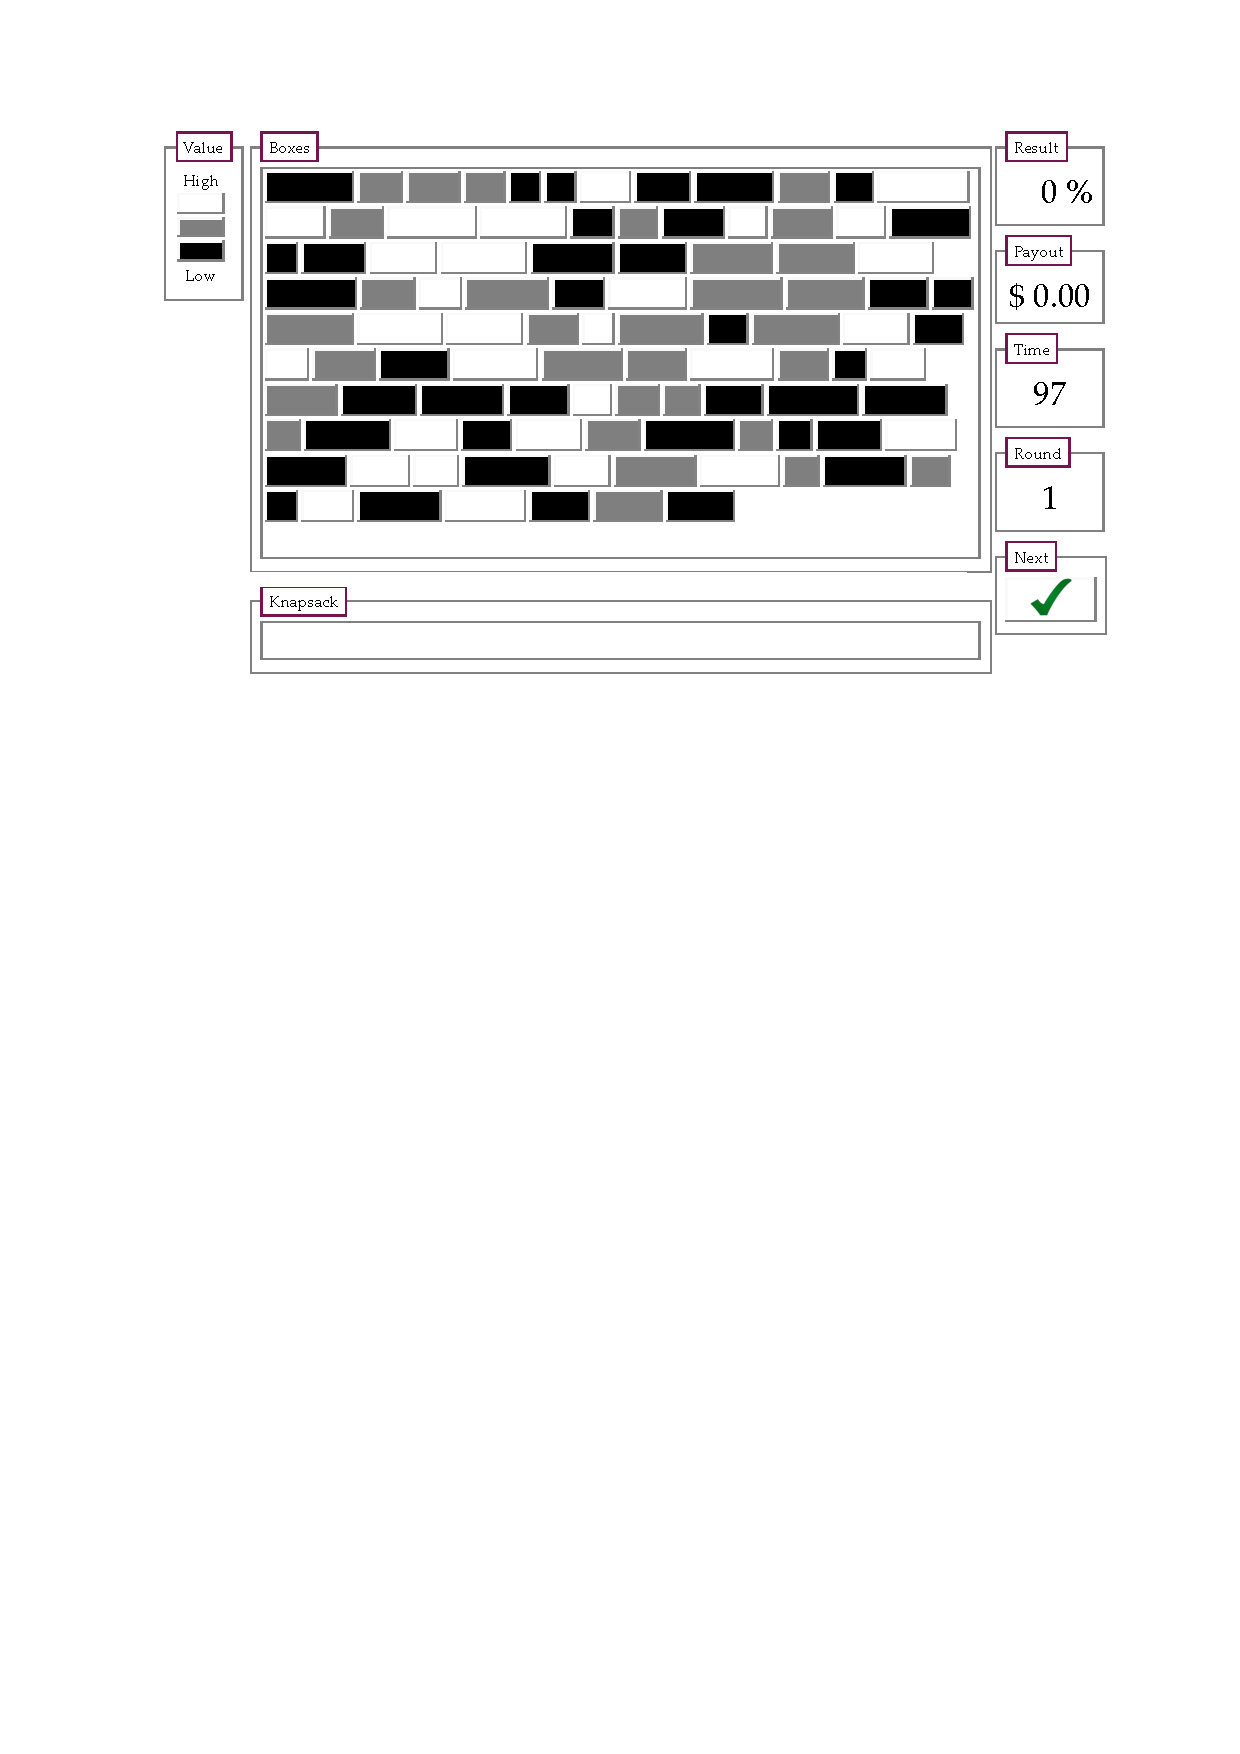
\includegraphics[height = 0.39\textwidth]{Interface1.pdf}
%\end{subfigure} 
%\begin{subfigure} 
%\centering
%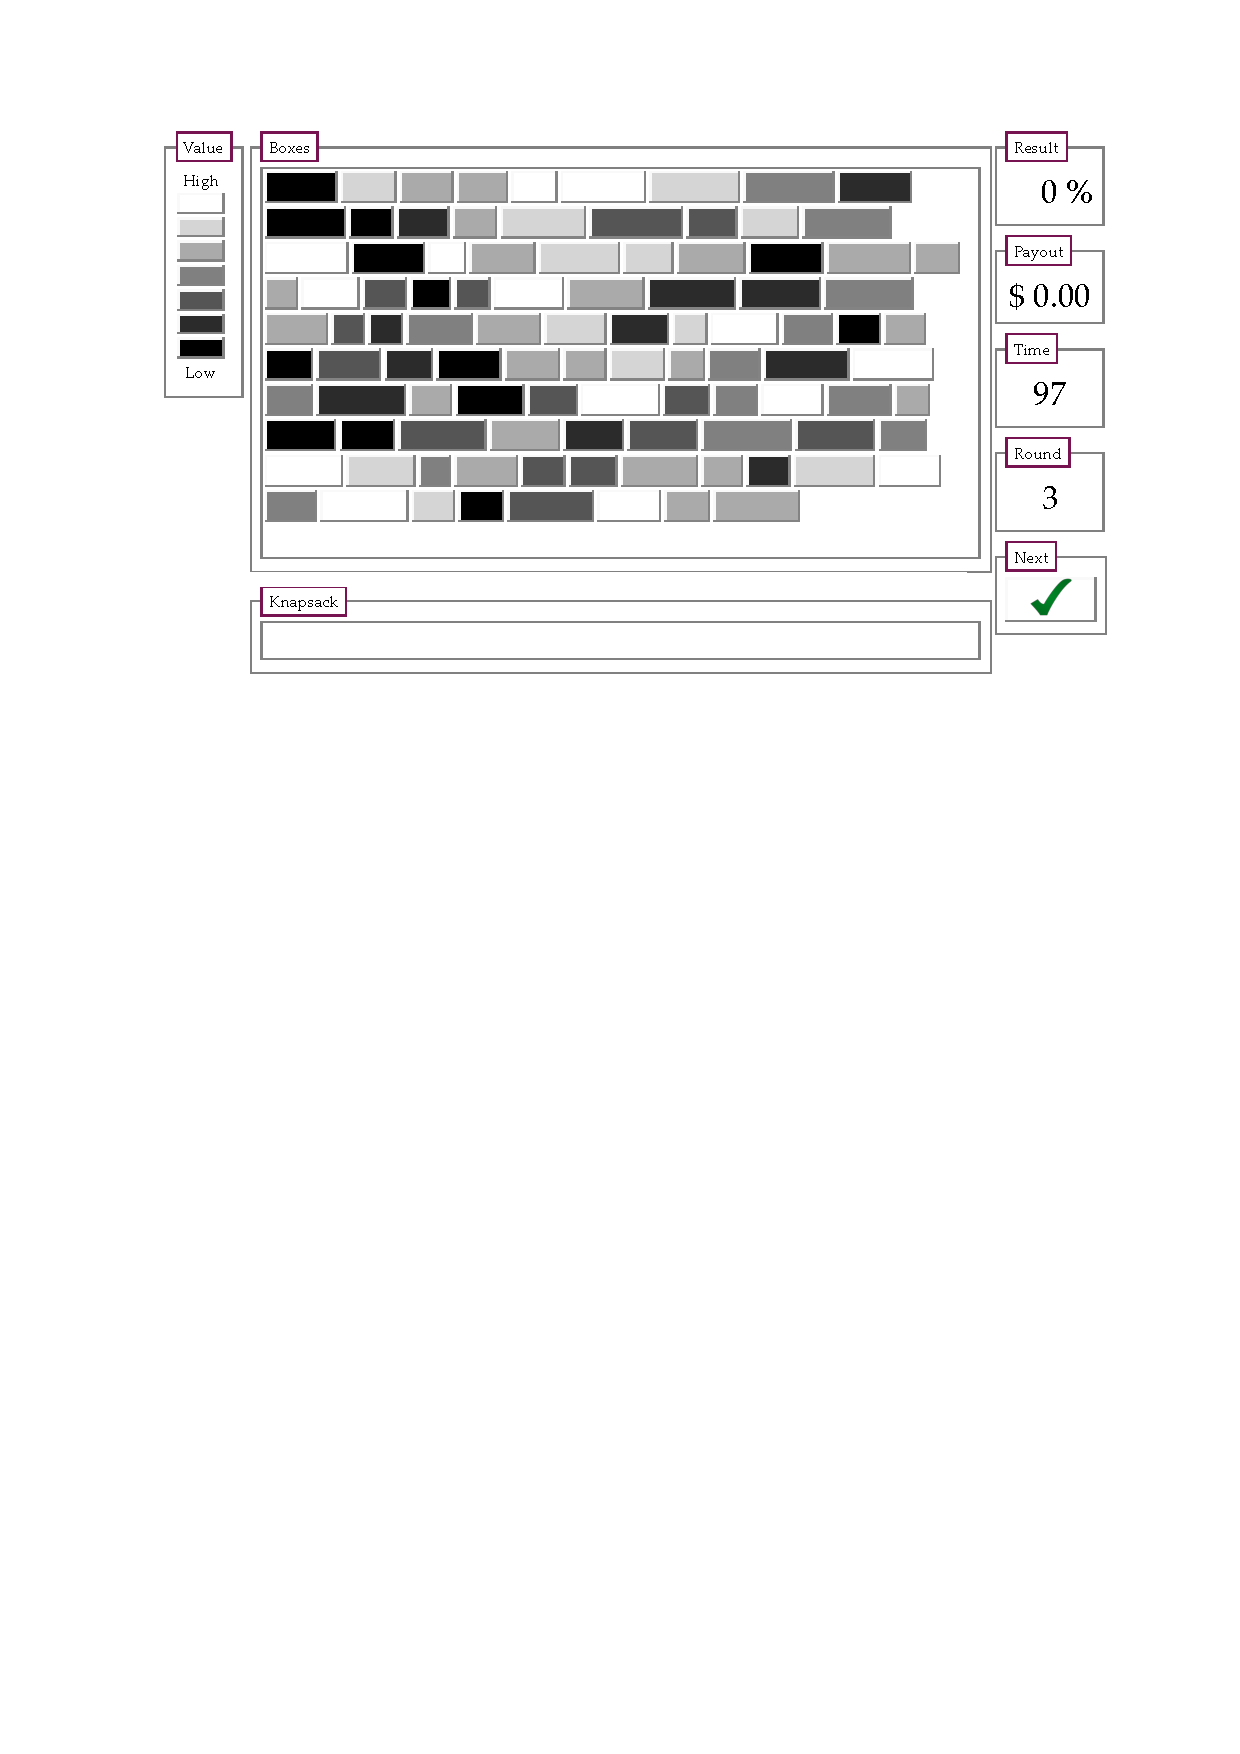
\includegraphics[height = 0.39\textwidth]{Interface2.pdf}
%\end{subfigure}
%\begin{subfigure} 
%\centering
%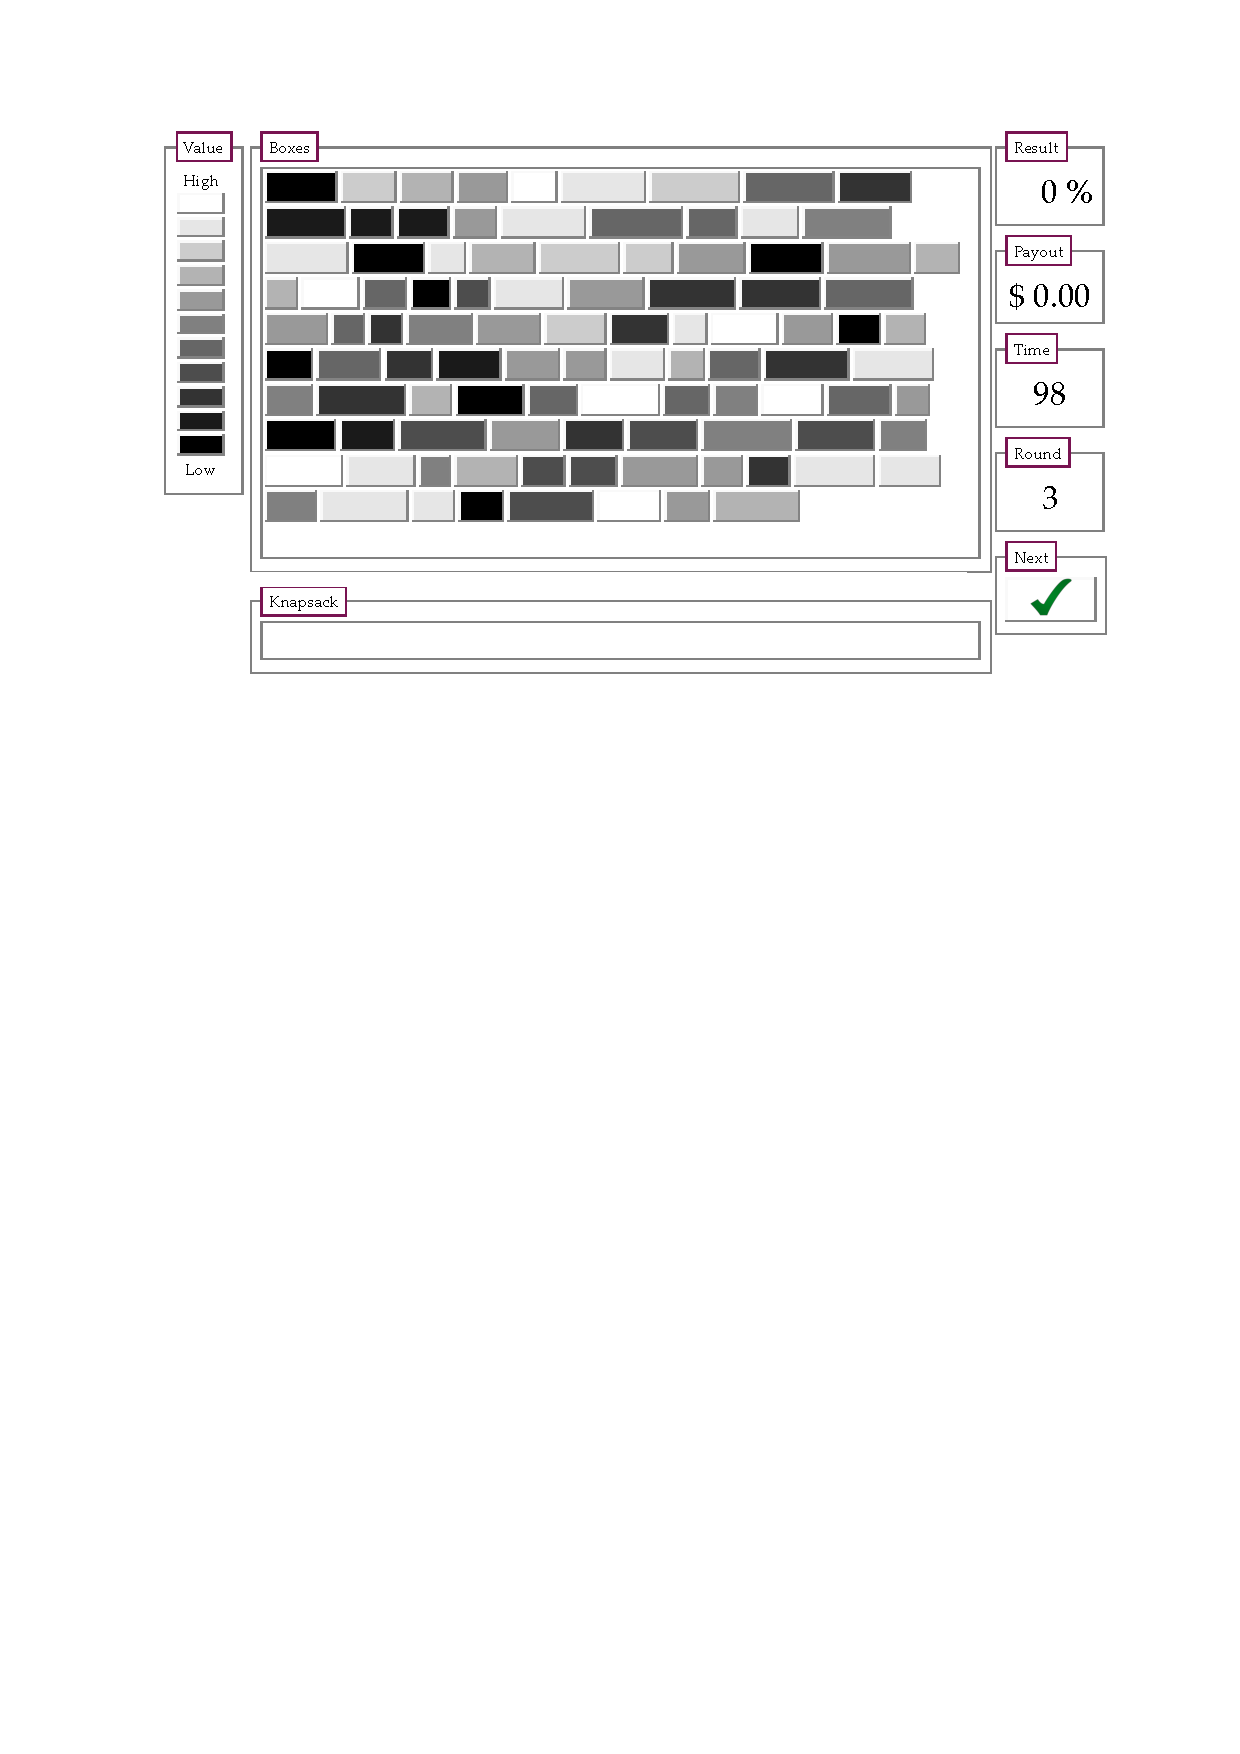
\includegraphics[height = 0.39\textwidth]{Interface3.pdf}
%\end{subfigure}
%  \caption{Interface for Usergroup 1, 2  and 3}
%    \label{InterfaceOverview} 
%\end{center}
%\end{figure}

\newpage

\section{Formulas}
		\label{Appendix-Formulas}

%\begin{figure}[htbp]
%\begin{equation}
%\begin{split}
%x' = \dfrac{1}{4}x+\dfrac{1}{4},\;x = 3,7,11,15\quad \quad \quad\\ 
%x := number\;of\;colours,\;x' := new\;variable
%\end{split}
%\end{equation}
%\caption{Number of colours - Usergroup}
%\label{NumberUsergroup}
%\end{figure}
\begin{equation}
\begin{split}
Share\;of\;dropout = \dfrac{p_i(user|dropout)}{p_i(user)}, \quad \quad \\ 
i = 1,..5,\;user := number\;of\;users\;logged\;in
\end{split}
\end{equation}

\begin{equation}
\begin{split}
Share\;of\;minimum\;payout = \dfrac{p_i(user|payout=0)}{p_i(user)}, \\ 
i = 1,..5,\;user := number\;of\;users \quad \quad
\end{split}
\end{equation}

%\begin{figure}[htbp]
%\caption{Box - Cox - Transformation}
%\label{BoxCoxTransformation}
\begin{equation}
y_i^{(\lambda)} = \begin{cases}
\dfrac{y_i^{\lambda}-1}{\lambda}, \quad if\;\lambda \neq 0, \\ 
log(y_i), \quad if\;\lambda = 0
\end{cases}, \quad y > 0 
\end{equation}

%\end{figure}

\section{Descriptive statistics}
		\label{Appendix-Descriptive}
		
\begin{figure}[htbp] % DistributionFirstResult
\begin{center} 
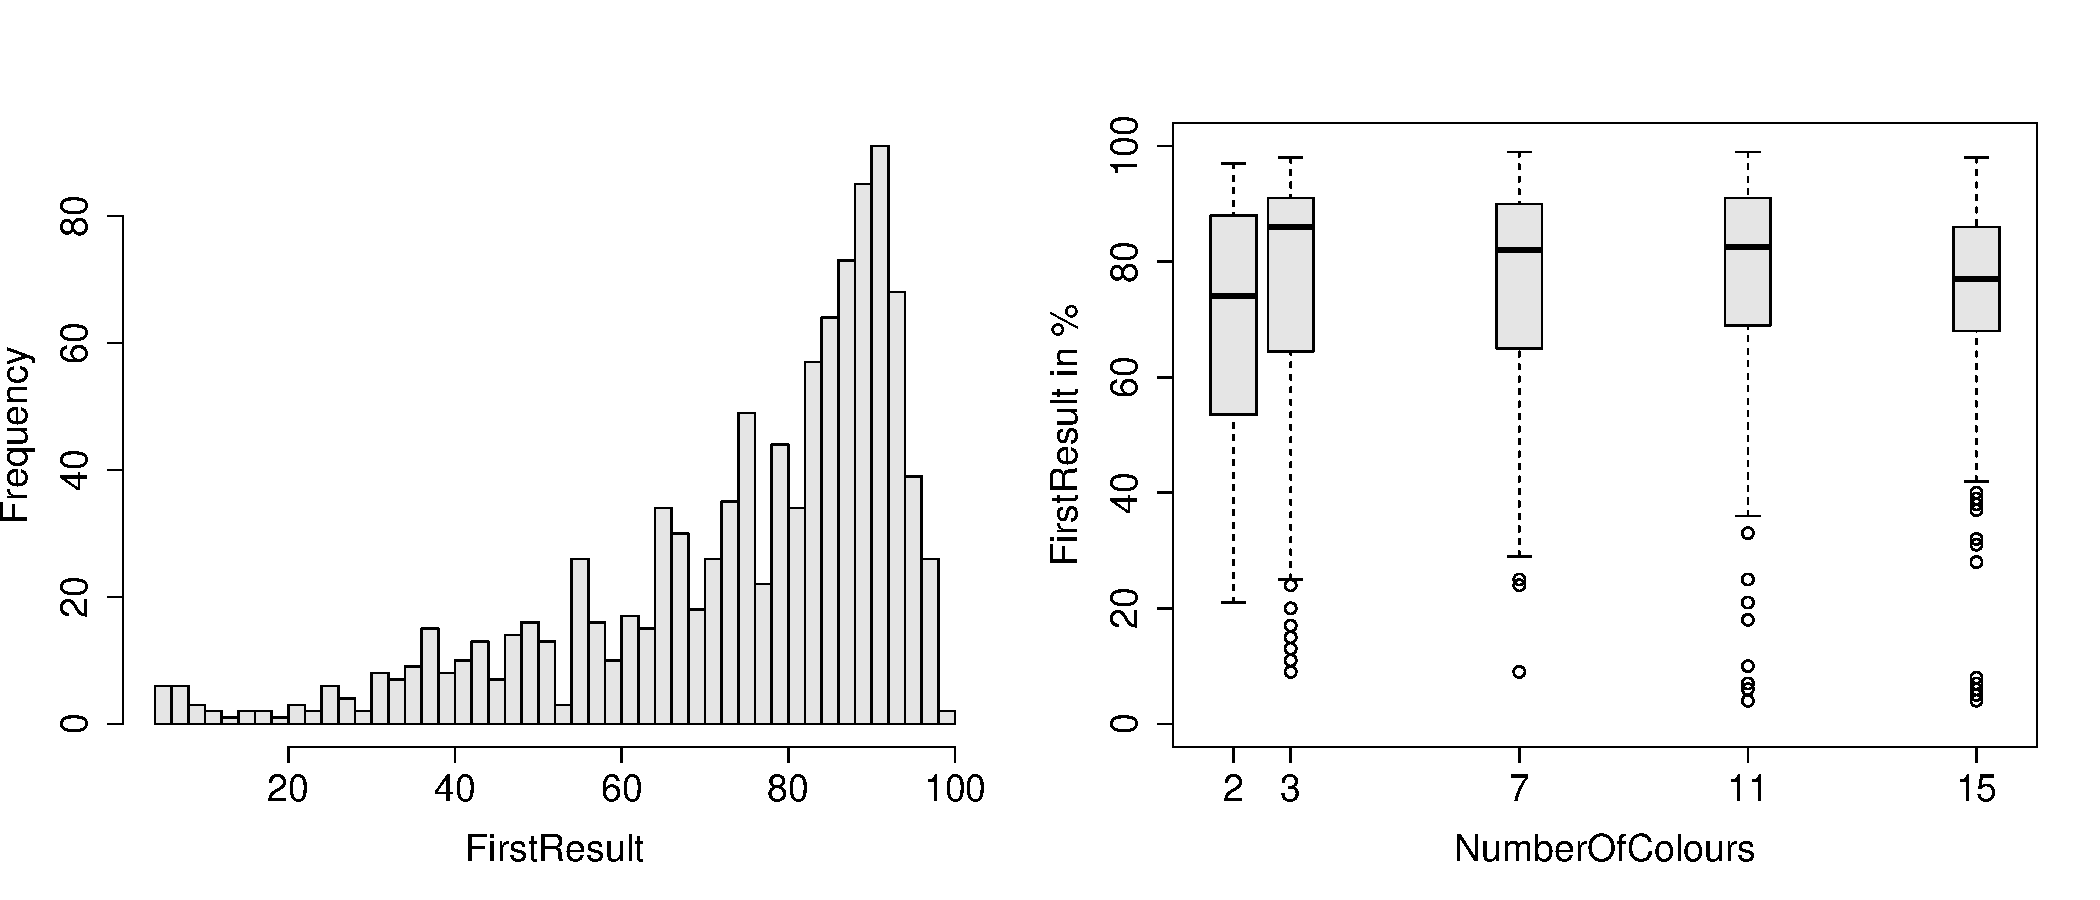
\includegraphics[height = 0.38\textwidth]{DescriptivesFirstResult.pdf}
  \caption{FirstResult - Histogram and Box plot}
    \label{DistributionFirstResult} 
\end{center}
\end{figure}

\begin{figure}[htbp] % DistributionBestResult
\begin{center} 
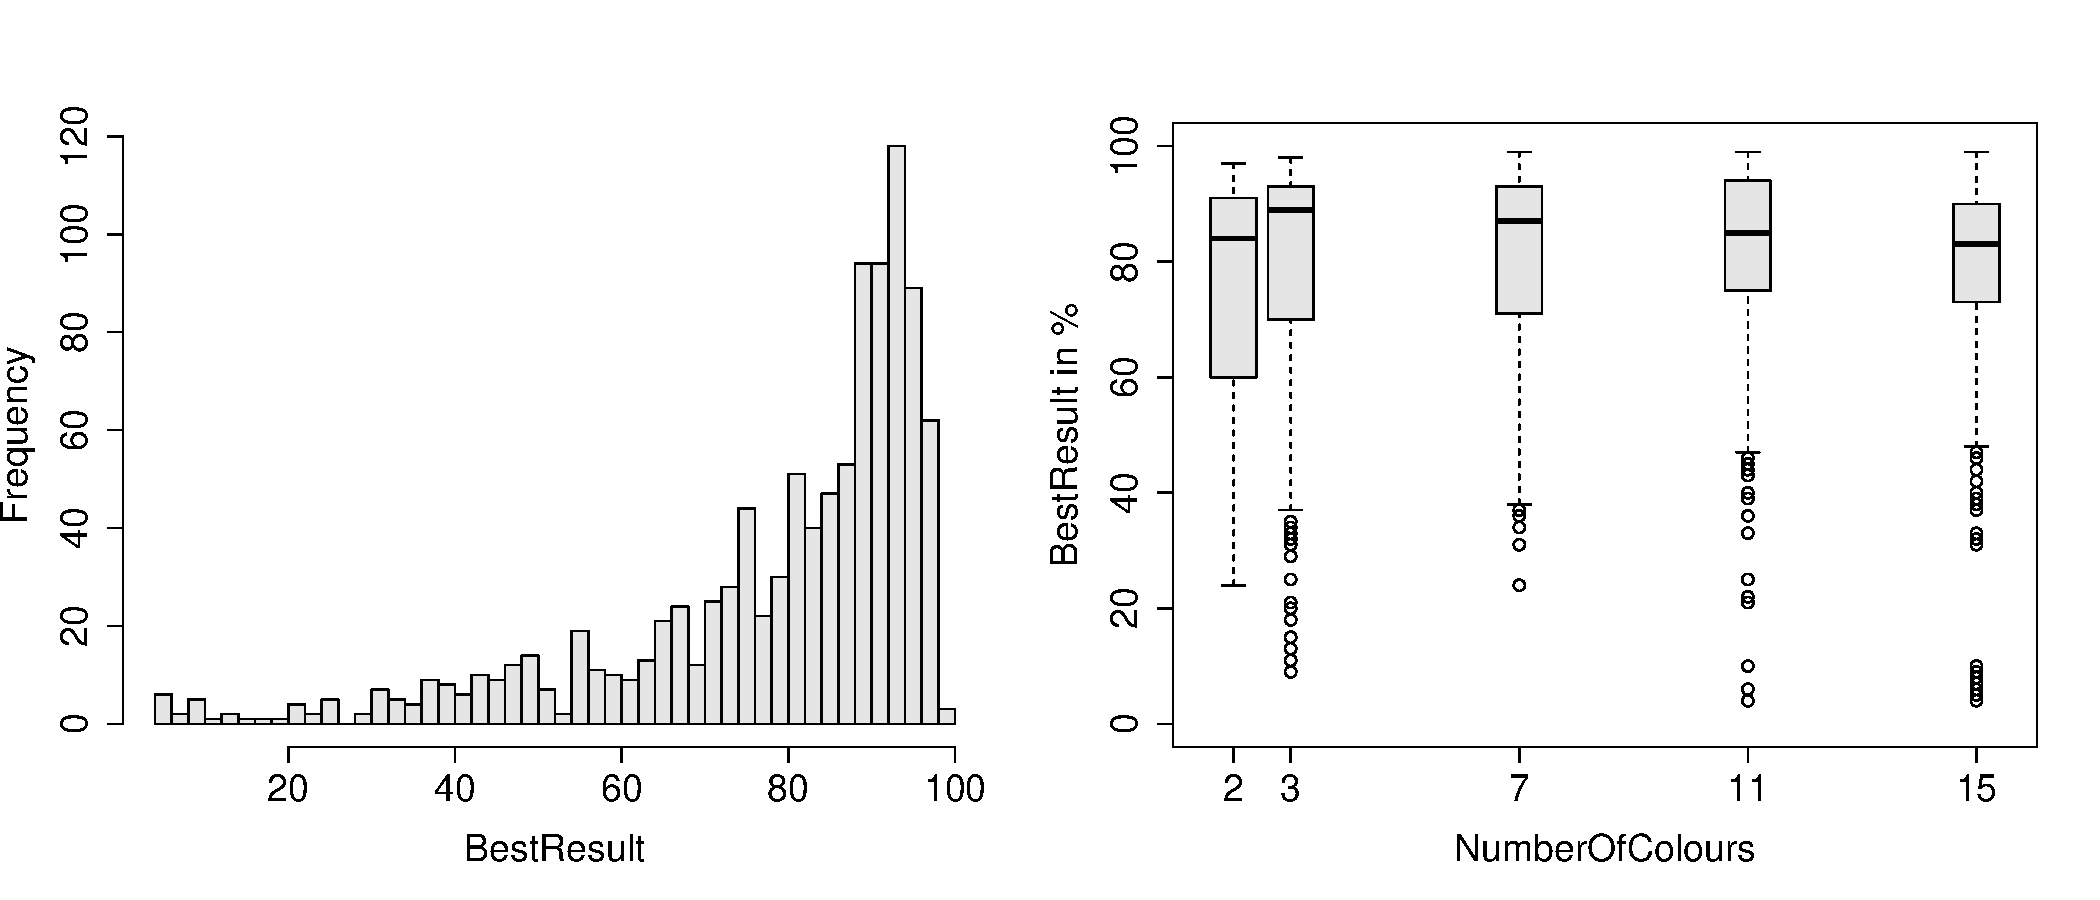
\includegraphics[height = 0.38\textwidth]{DescriptivesBestResult.pdf}
  \caption{BestResult - Histogram and Box plot}
    \label{DistributionBestResult} 
\end{center}
\end{figure}

\begin{figure}[htbp] % DistributionFirstTime
\begin{center} 
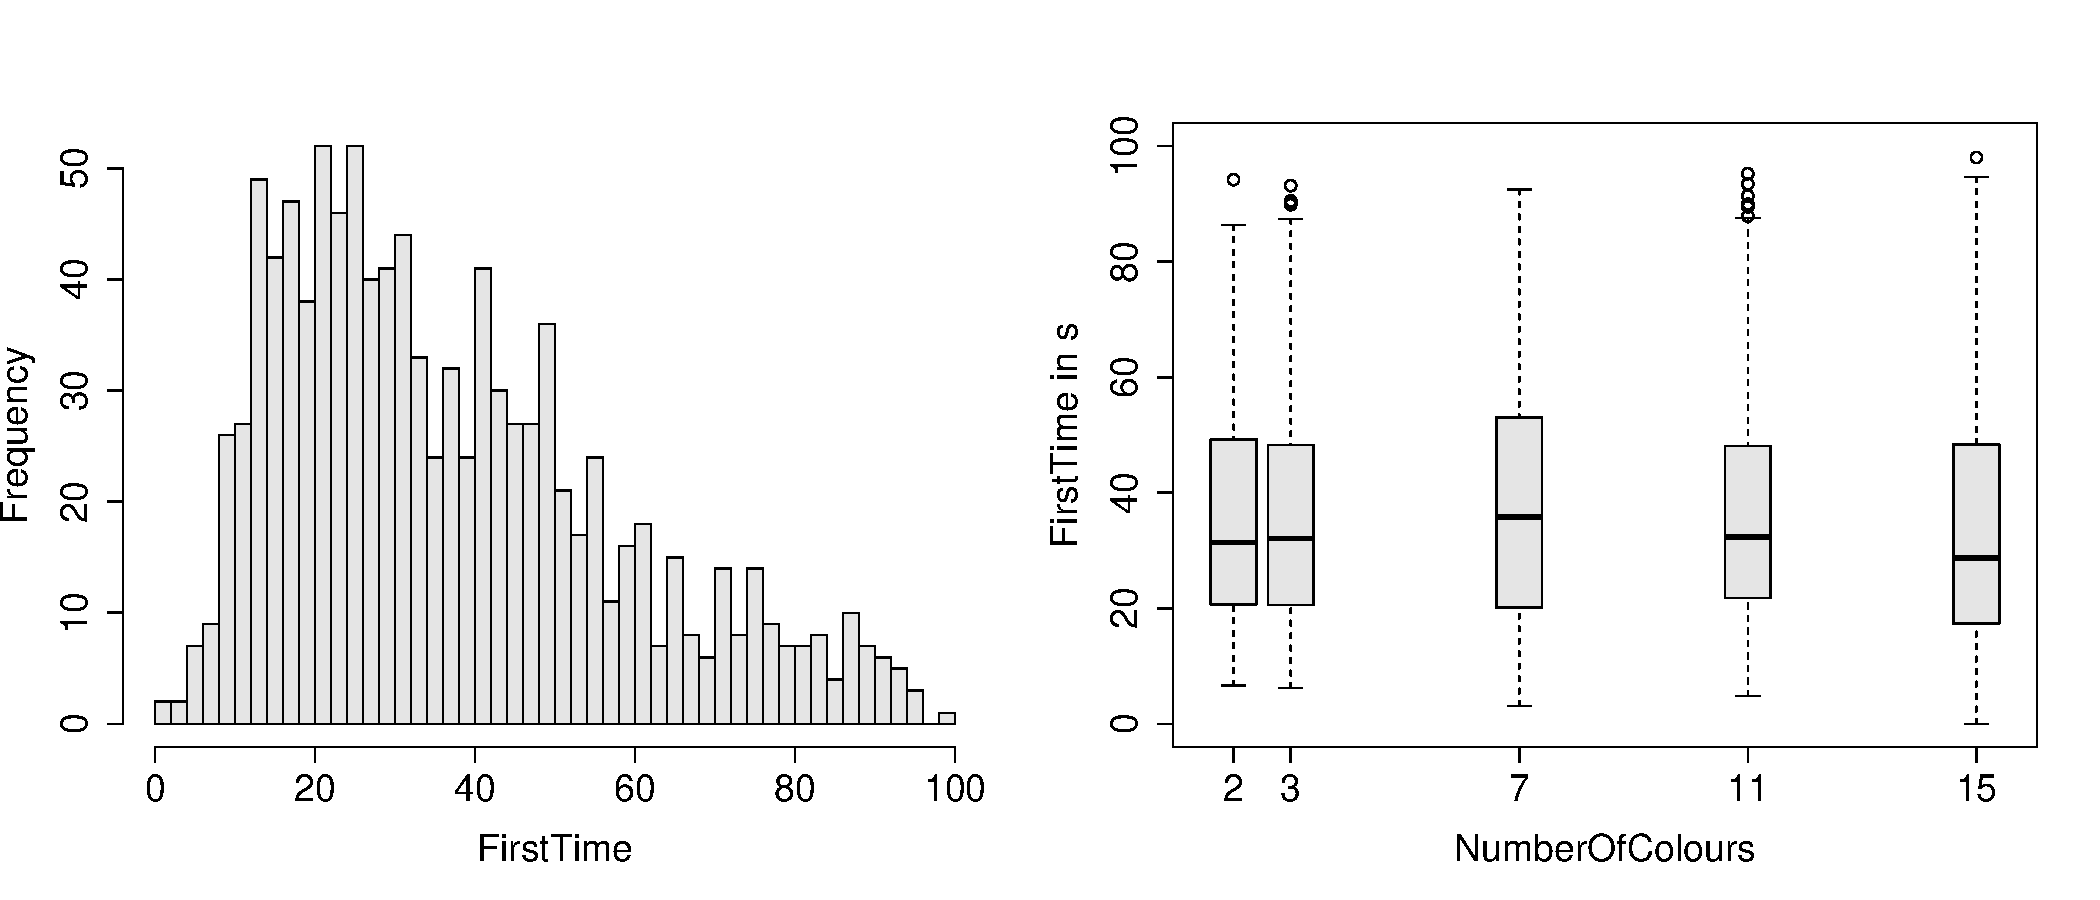
\includegraphics[height = 0.38\textwidth]{DescriptivesFirstTime.pdf}
  \caption{FirstTime - Histogram and Box plot}
    \label{DistributionFirstTime} 
\end{center}
\end{figure}
\begin{figure}[htbp] % DistributionBestTime
\begin{center} 
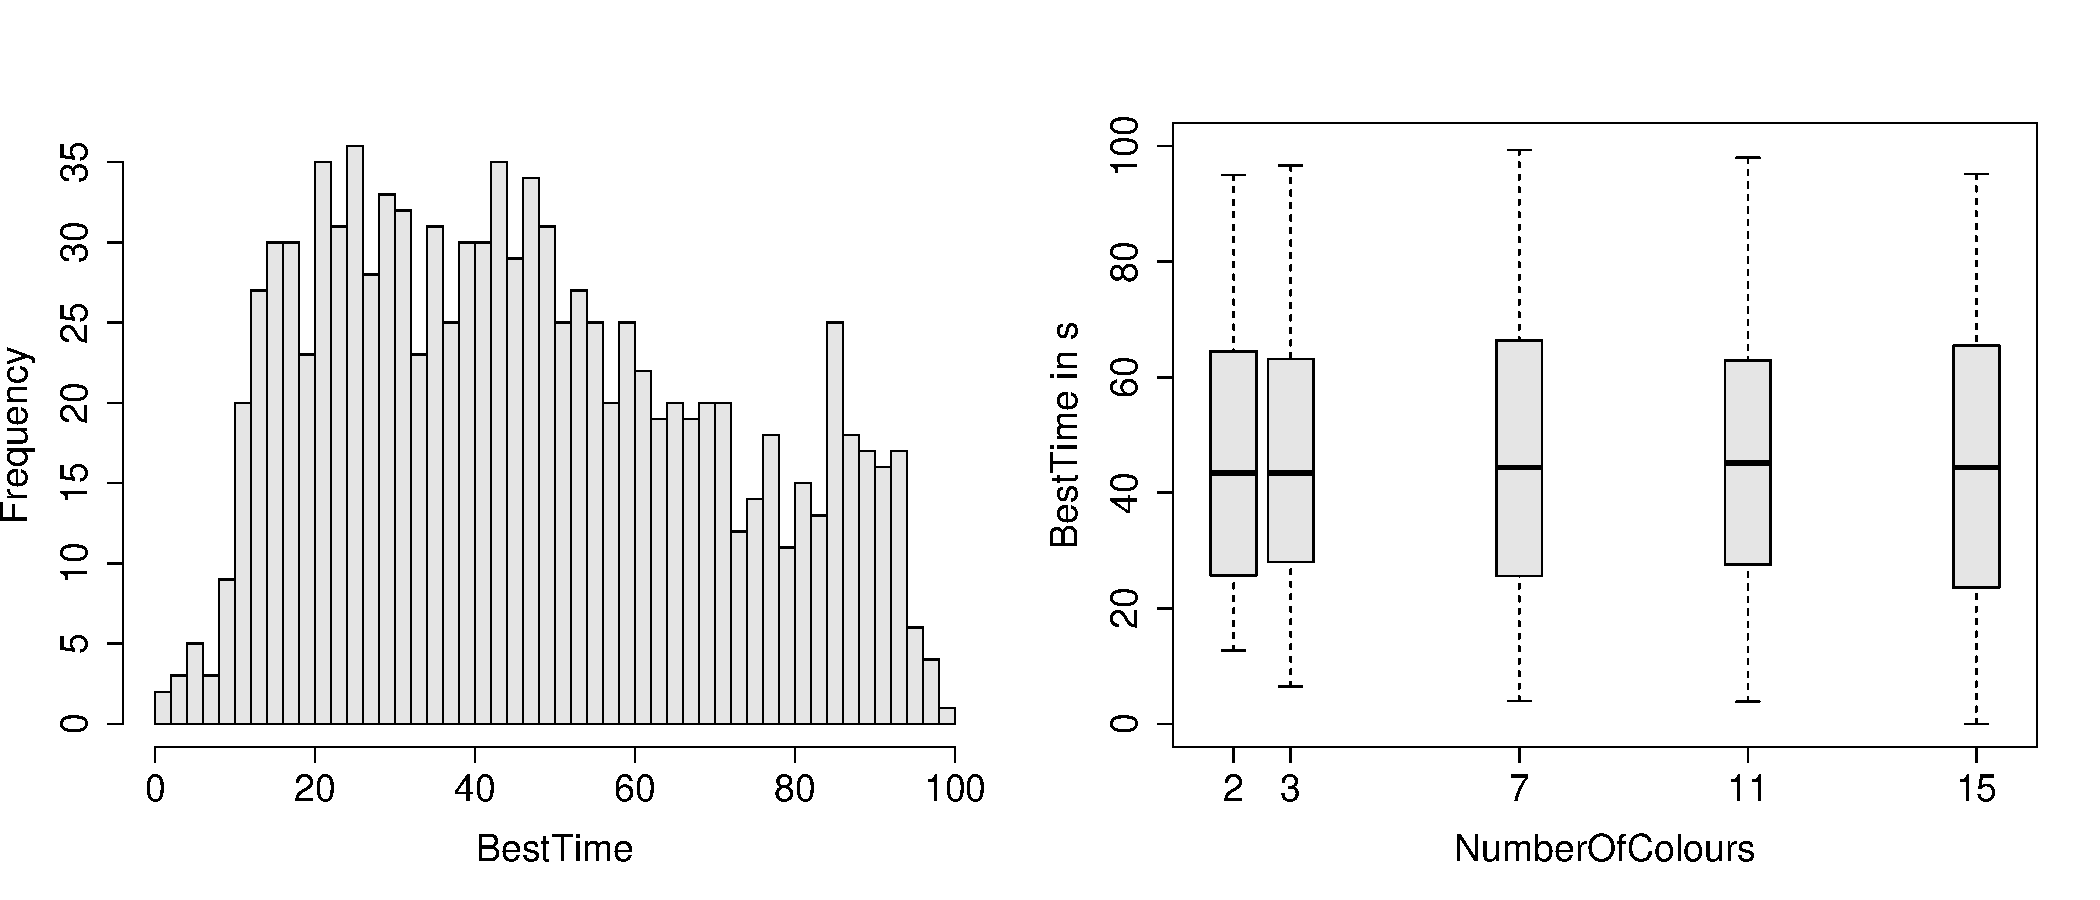
\includegraphics[height = 0.38\textwidth]{DescriptivesBestTime.pdf}
  \caption{BestTime - Histogram and Box plot}
    \label{DistributionBestTime} 
\end{center}
\end{figure}

\begin{figure}[htbp] % DistributionDecisionTime
\begin{center} 
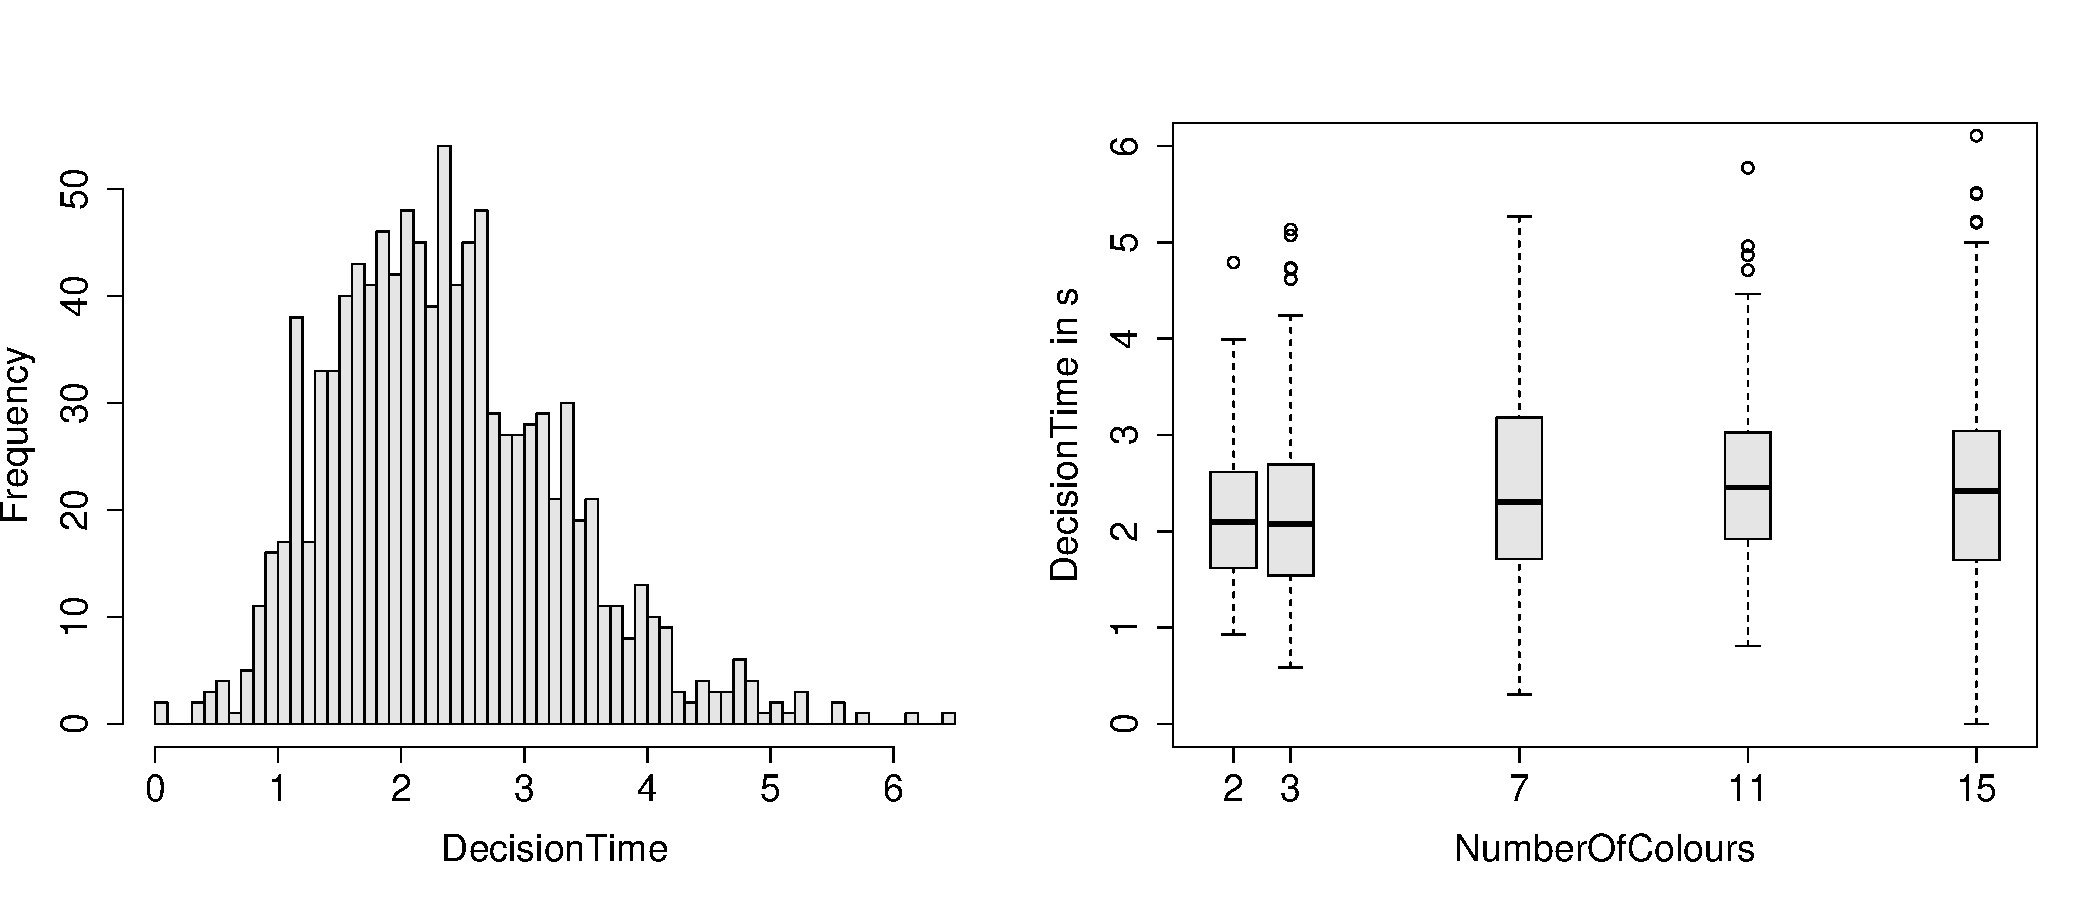
\includegraphics[height = 0.38\textwidth]{DescriptivesDecisionTime.pdf}
  \caption{DecisionTime - Histogram and Box plot}
    \label{DistributionDecisionTime} 
\end{center}
\end{figure}

\begin{figure}[htbp] % Question1
\centering
  \caption[Question 1 - Histogram and Box plot]{Question 1 - very low (1) to very high (7)}
    \label{Question1}  
\begin{subfigure} 
\centering
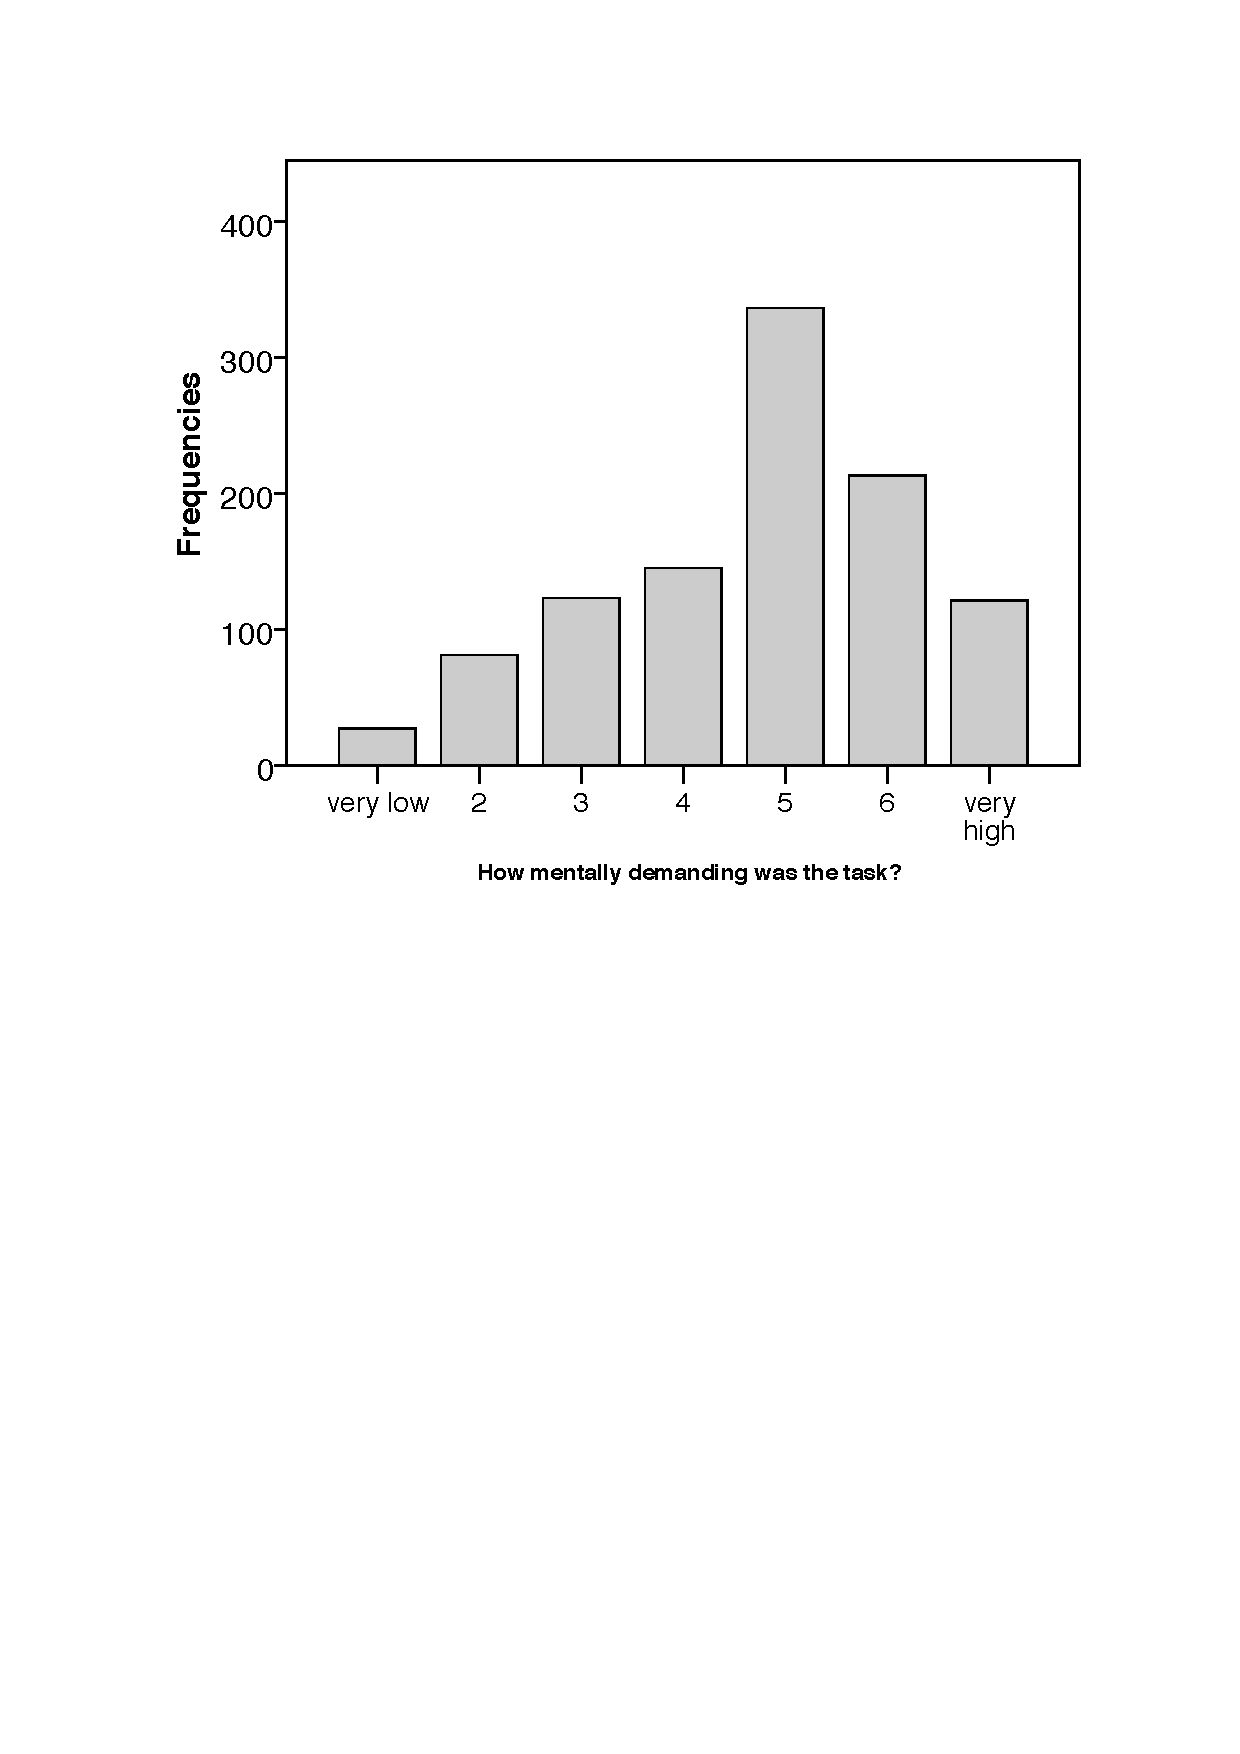
\includegraphics[height = 0.38\textwidth]{HistogramQuestion1.pdf}
\end{subfigure} 
\begin{subfigure} 
\centering
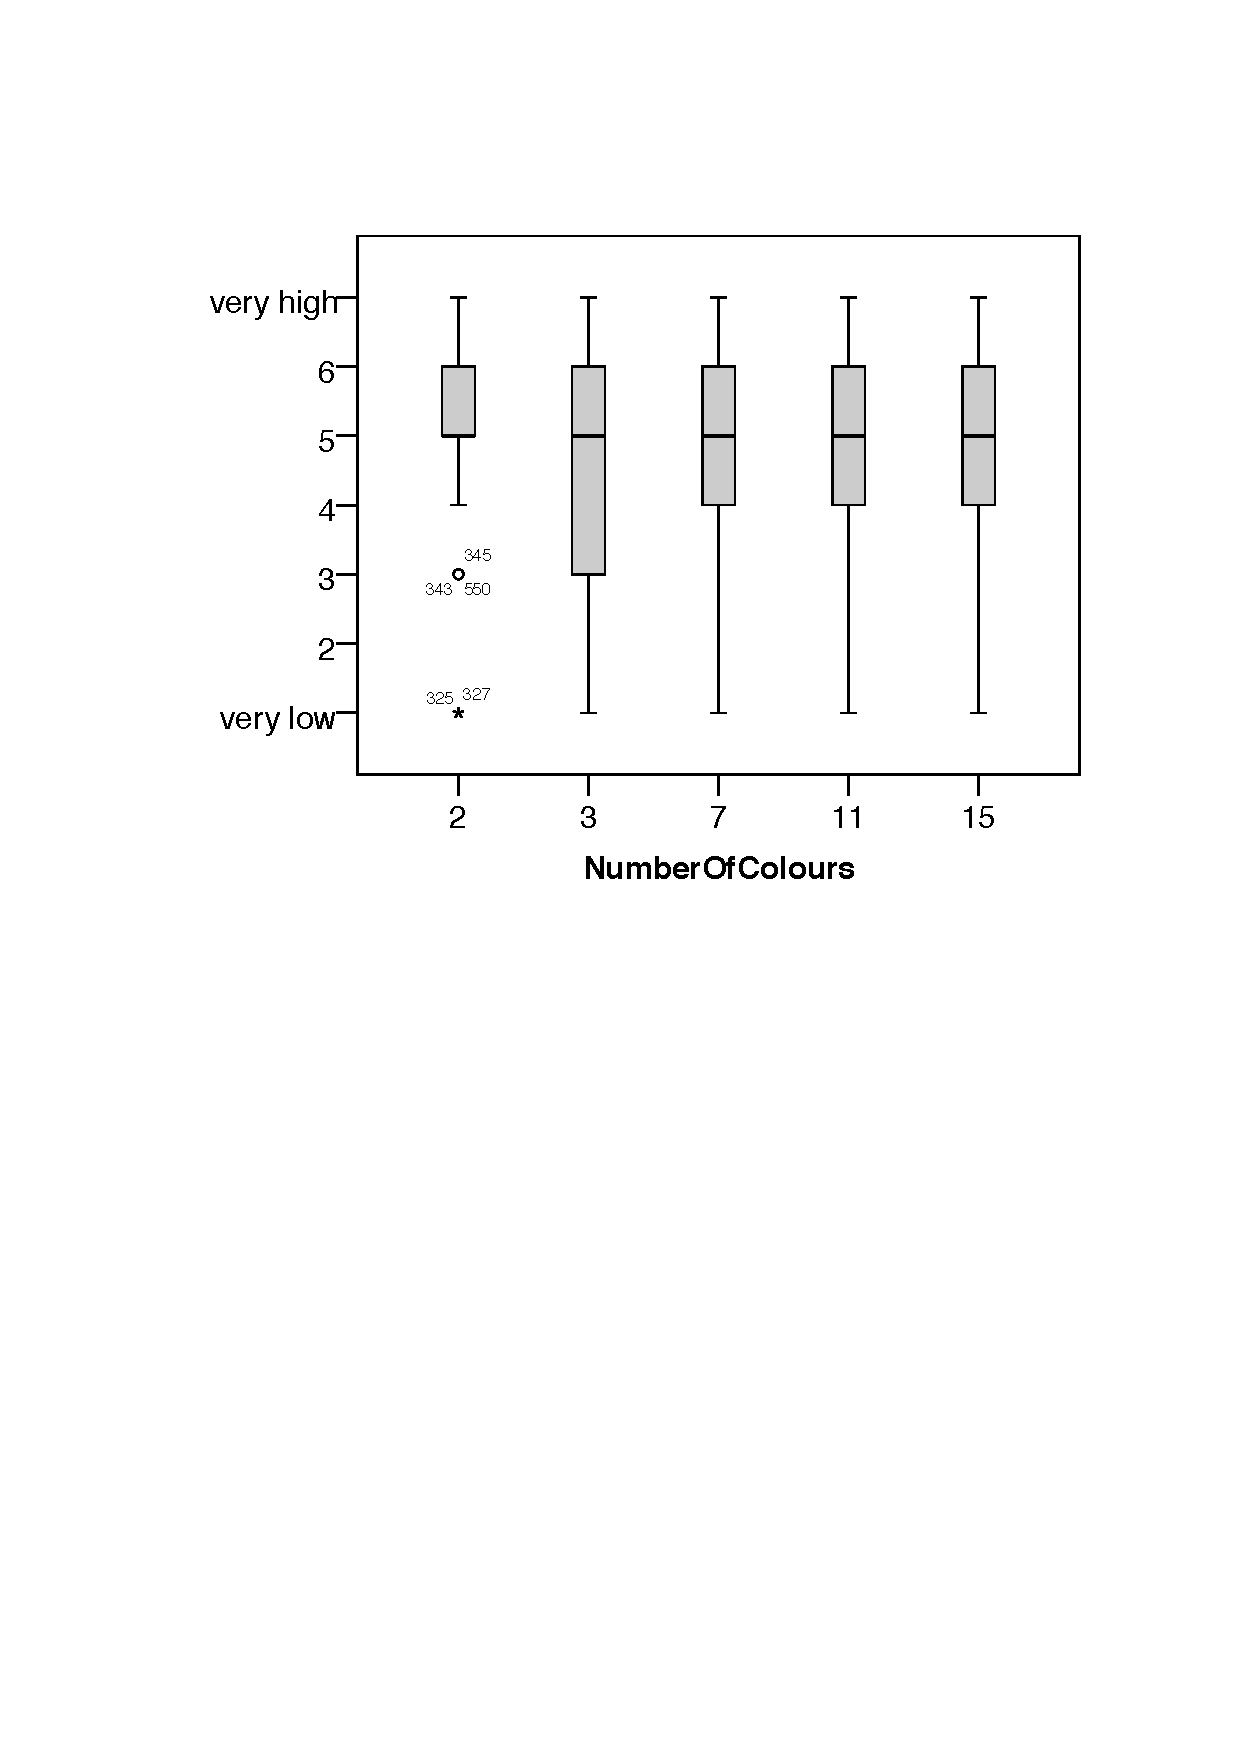
\includegraphics[height = 0.38\textwidth]{BoxplotQuestion1.pdf}
\end{subfigure}
\end{figure}
\begin{figure}[htbp] % Question2	
\begin{center} 
\begin{subfigure} 
\centering
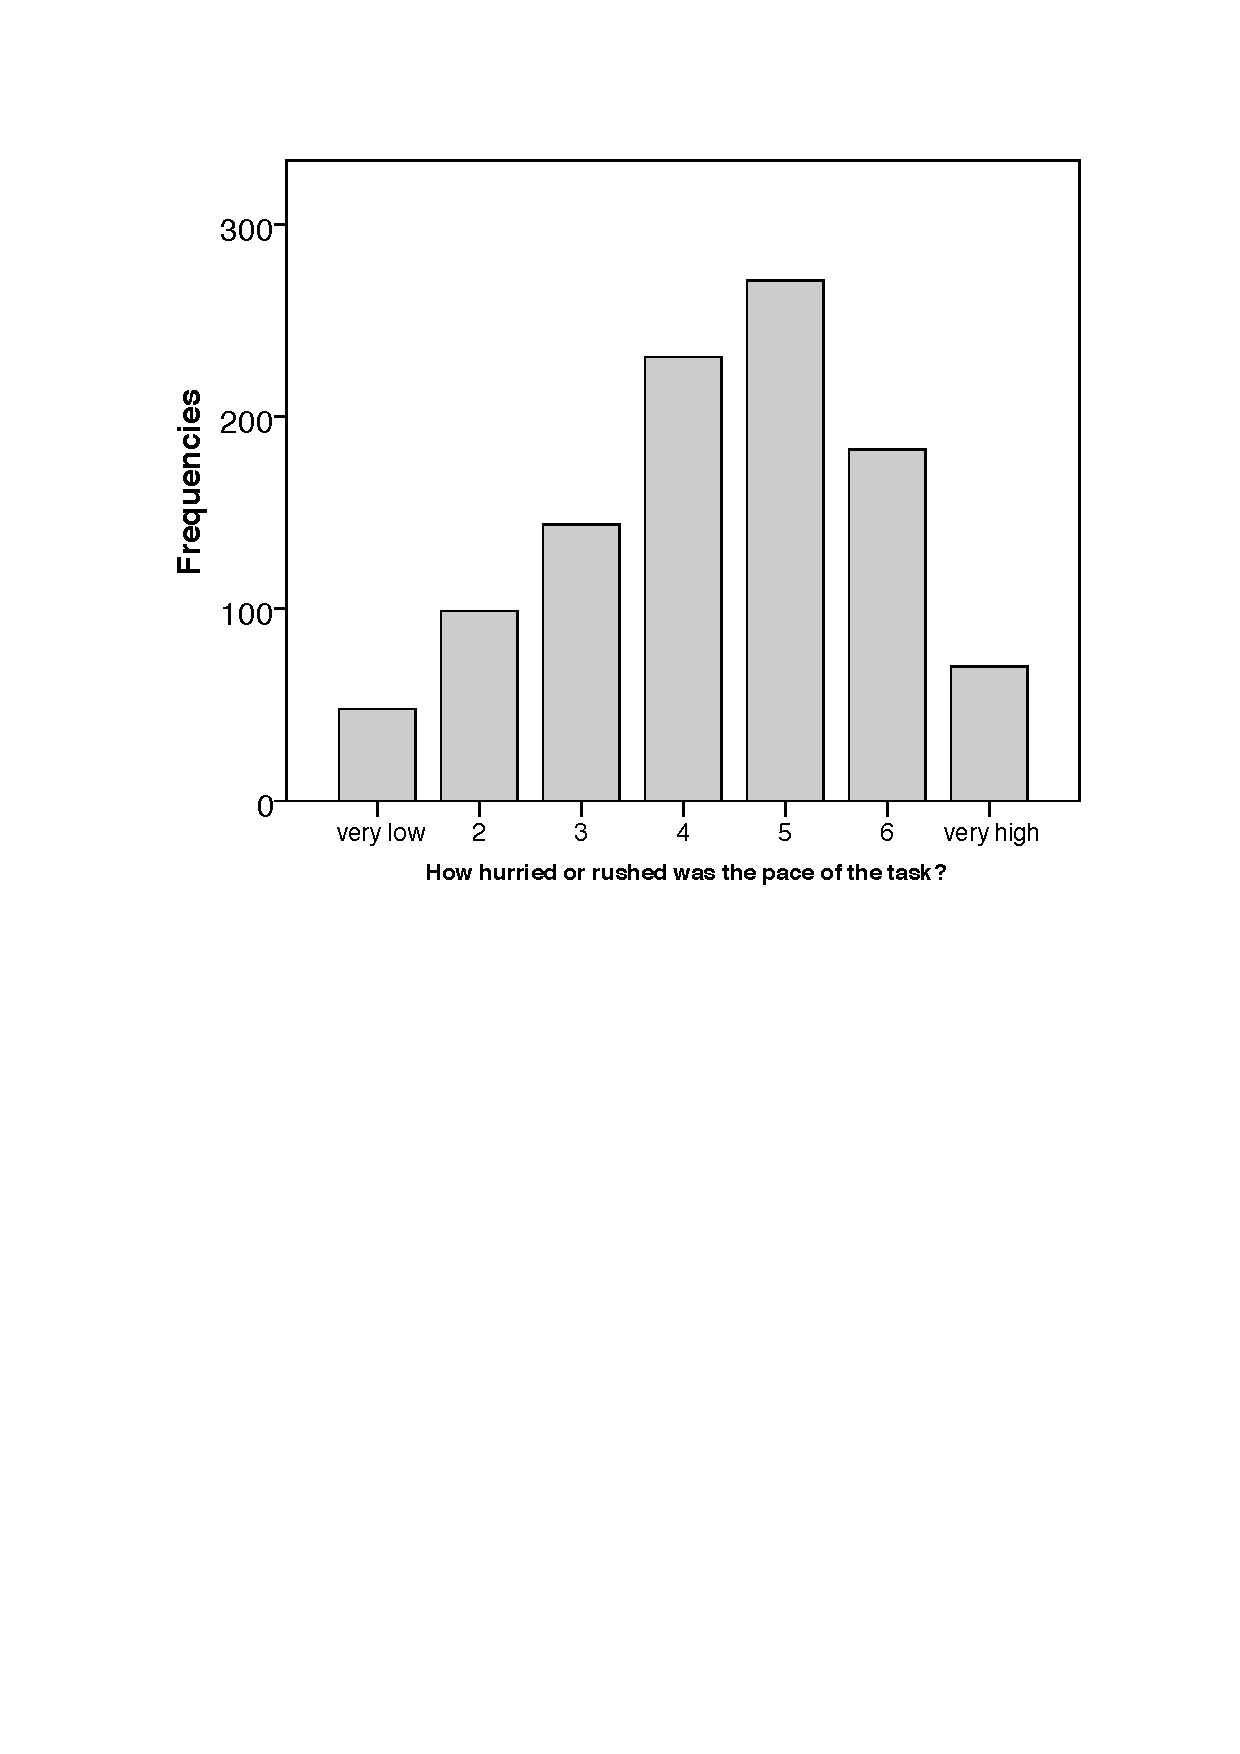
\includegraphics[height = 0.38\textwidth]{HistogramQuestion2.pdf}
\end{subfigure} 
\begin{subfigure} 
\centering
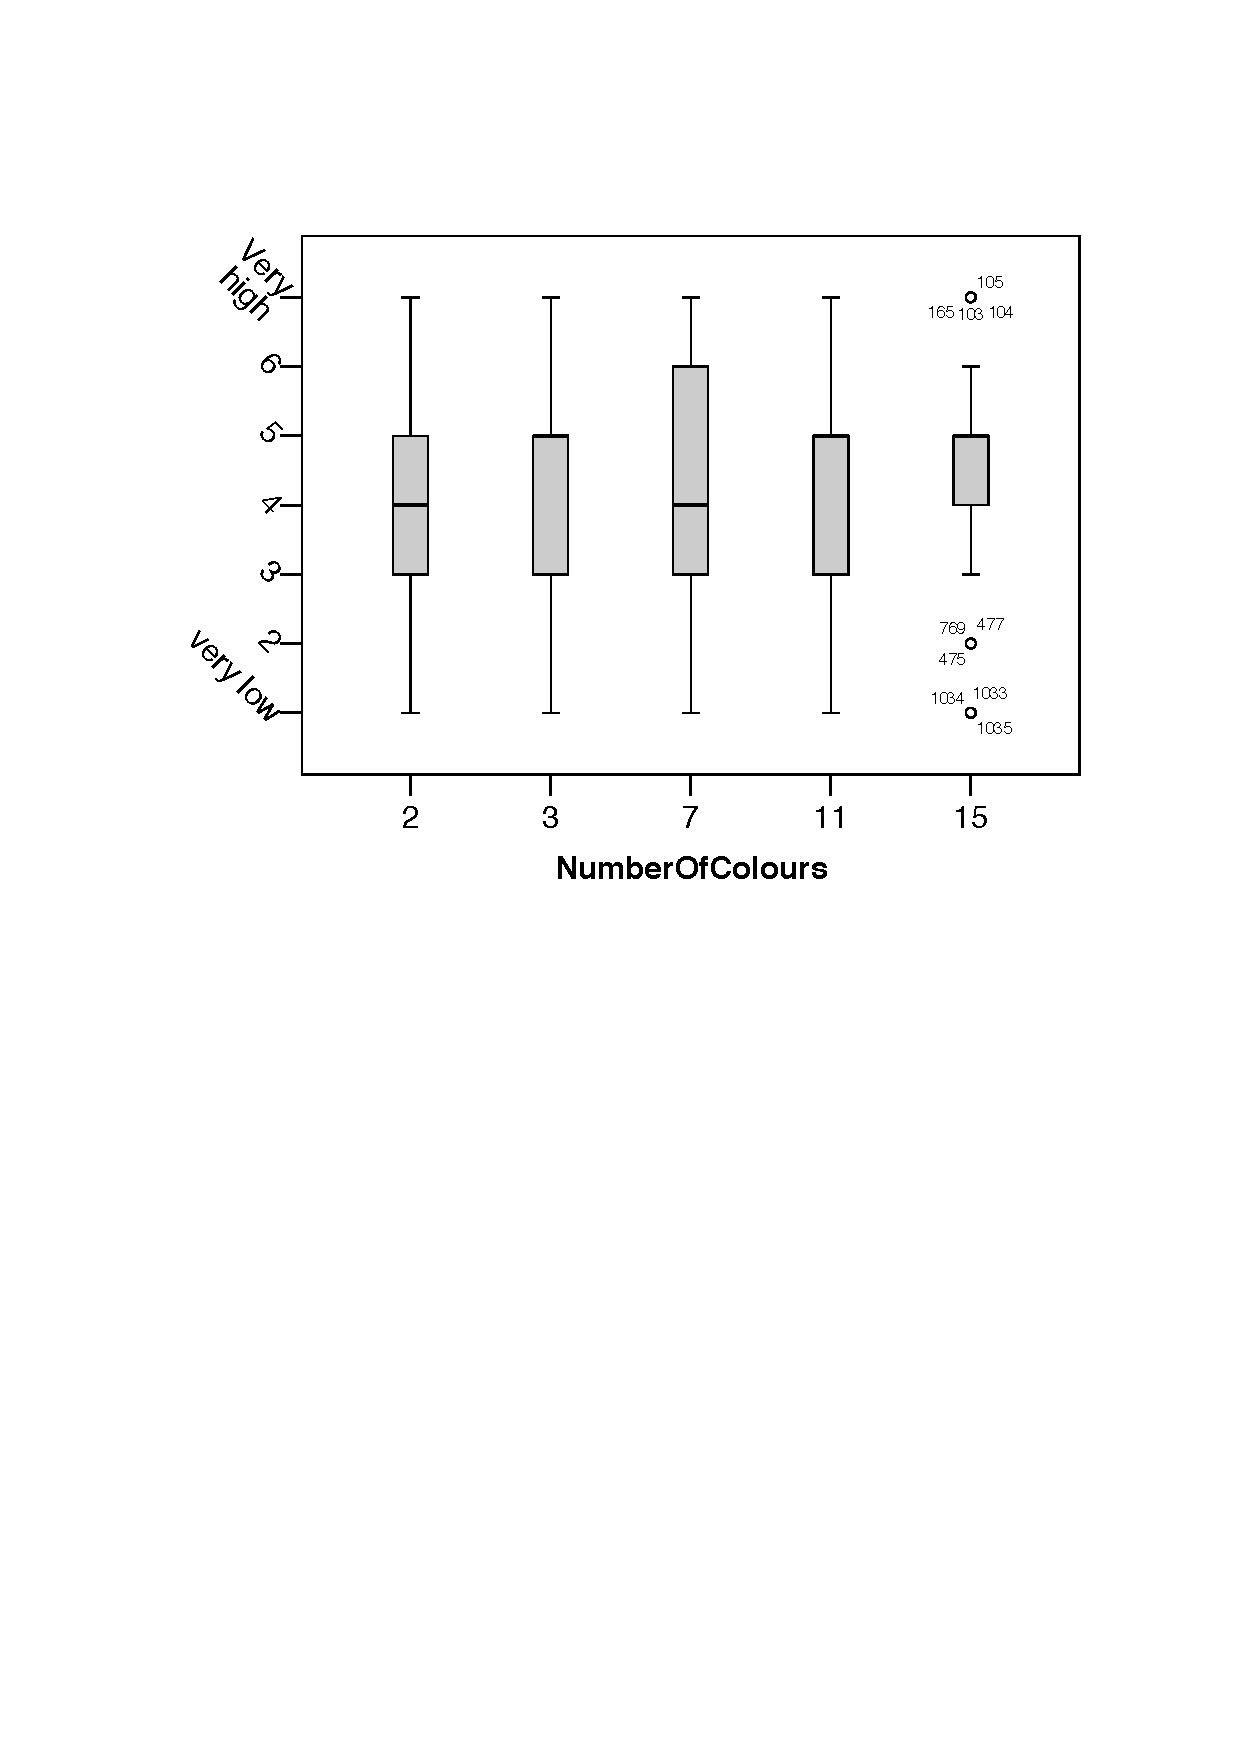
\includegraphics[height = 0.38\textwidth]{BoxplotQuestion2.pdf}
\end{subfigure}
  \caption[Question 2 - Histogram and Box plot]{Question 2 - very low (1) to very high (7)}
    \label{Question2} 
\end{center}
\end{figure}
\begin{figure}[htbp] % Question3	
\begin{center} 
\begin{subfigure} 
\centering
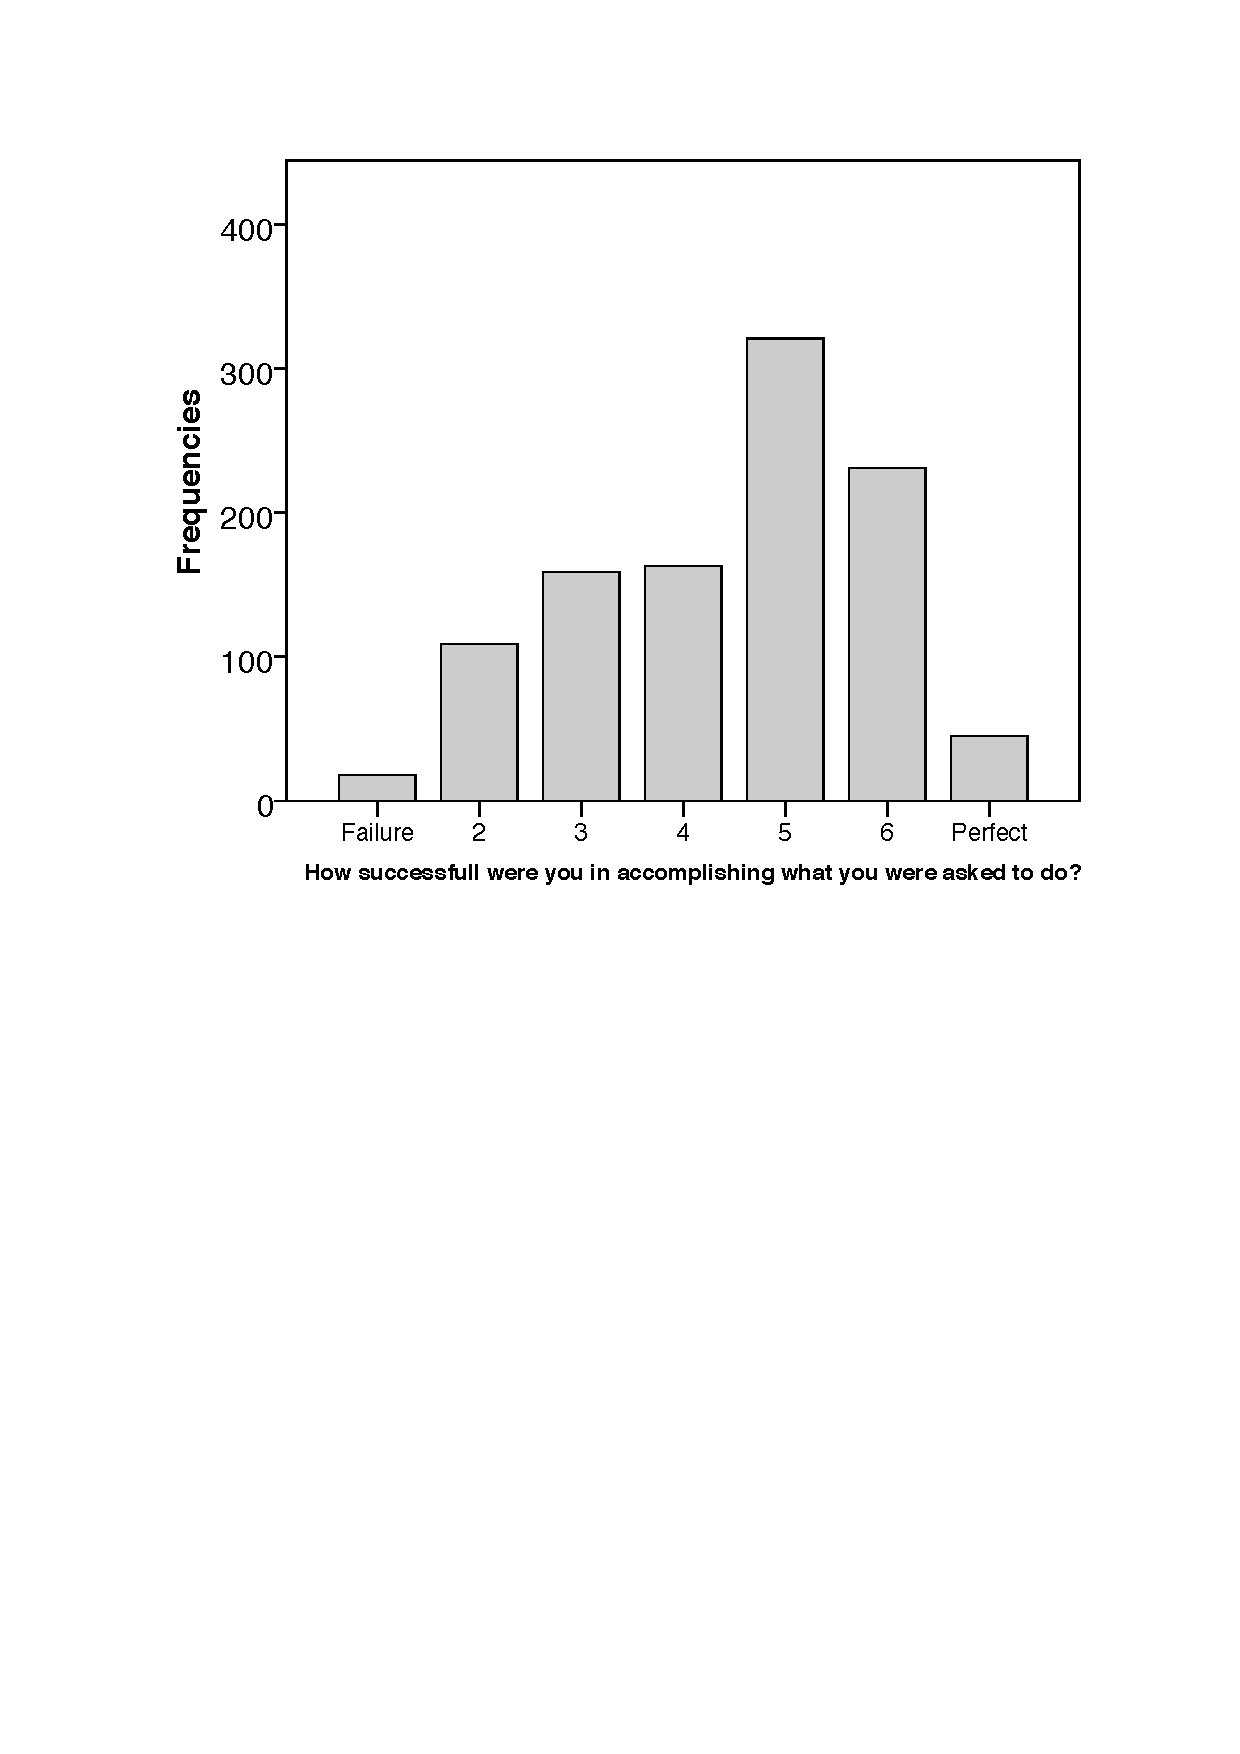
\includegraphics[height = 0.35\textwidth]{HistogramQuestion3.pdf}
\end{subfigure} 
\begin{subfigure} 
\centering
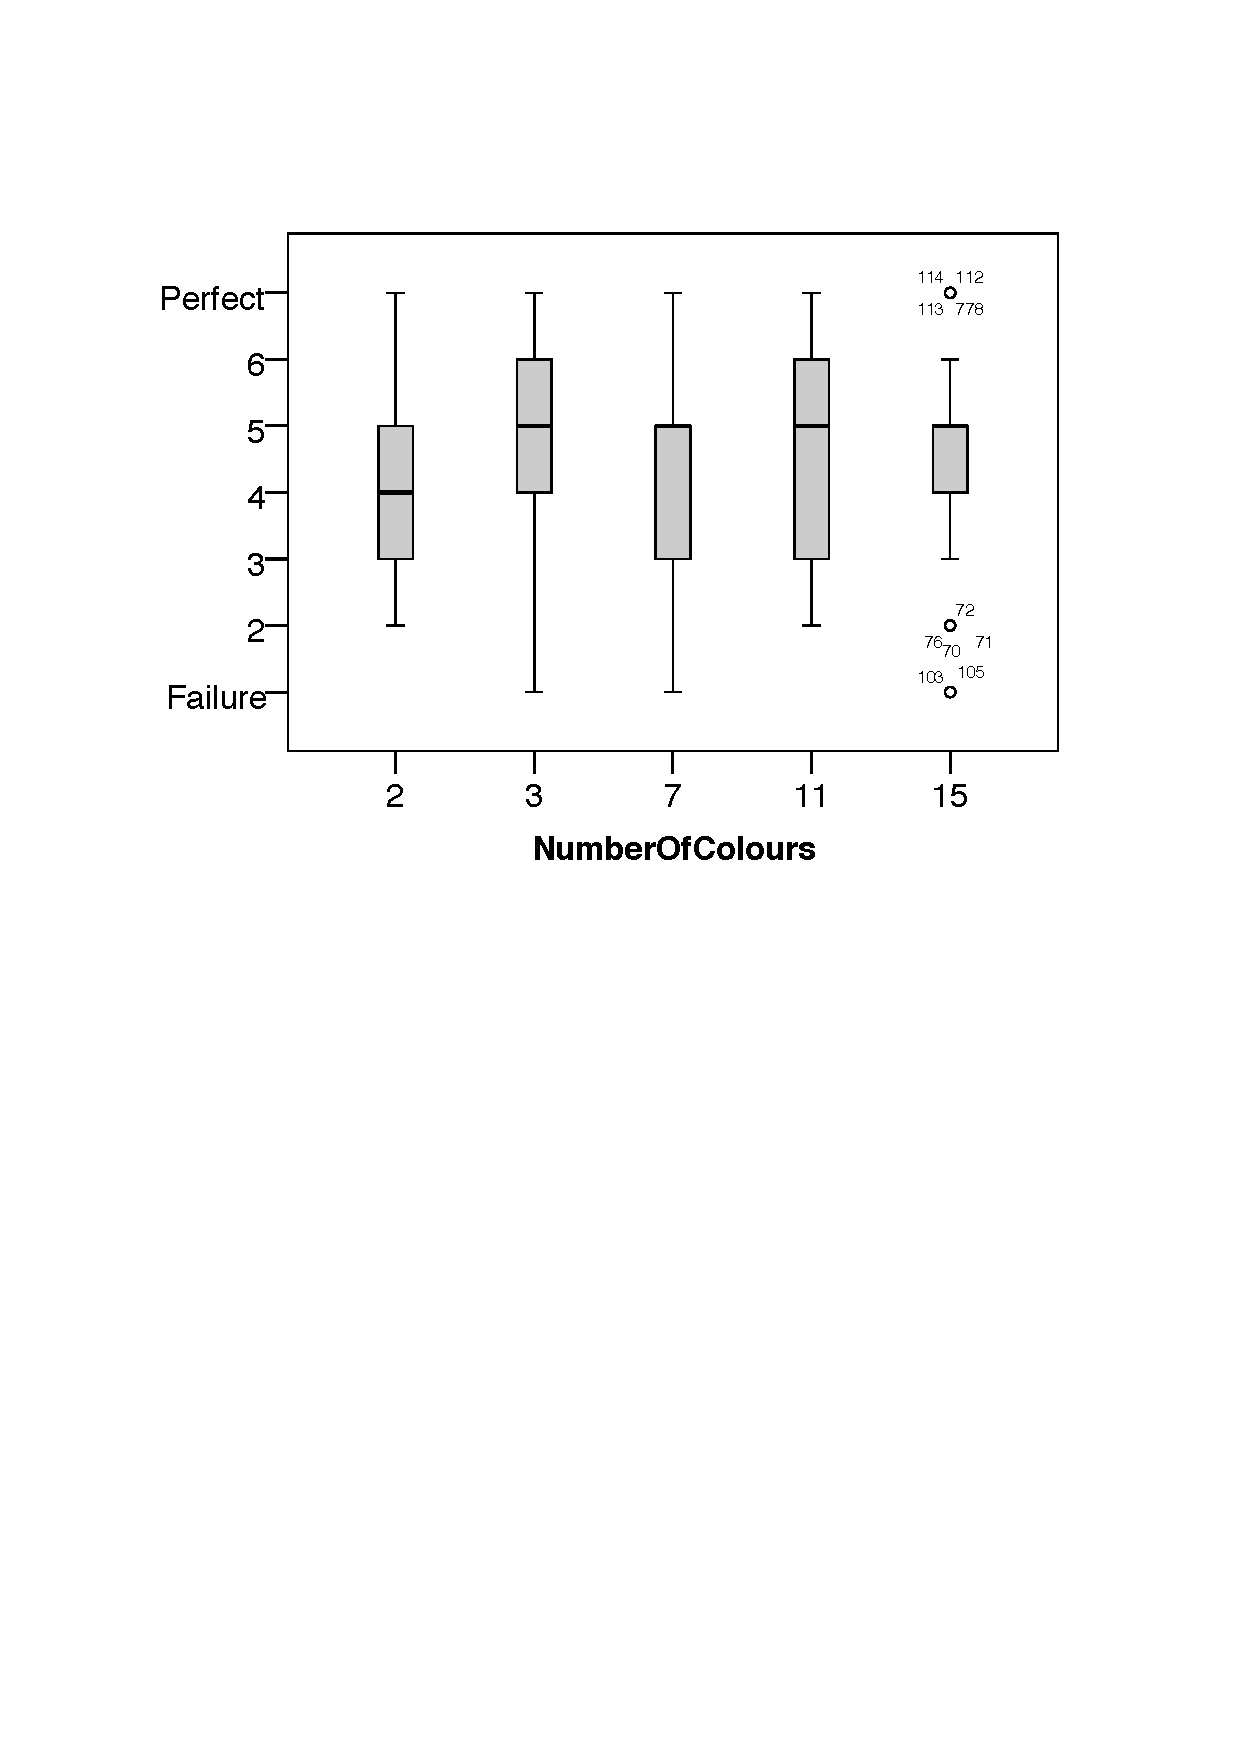
\includegraphics[height = 0.35\textwidth]{BoxplotQuestion3.pdf}
\end{subfigure}
  \caption[Question 3 - Histogram and Box plot]{Question 3 - Failure (1) to Perfect (7)}
    \label{Question3} 
\end{center}
\end{figure}
\begin{figure}[htbp] % Question4	
\begin{center} 
\begin{subfigure} 
\centering
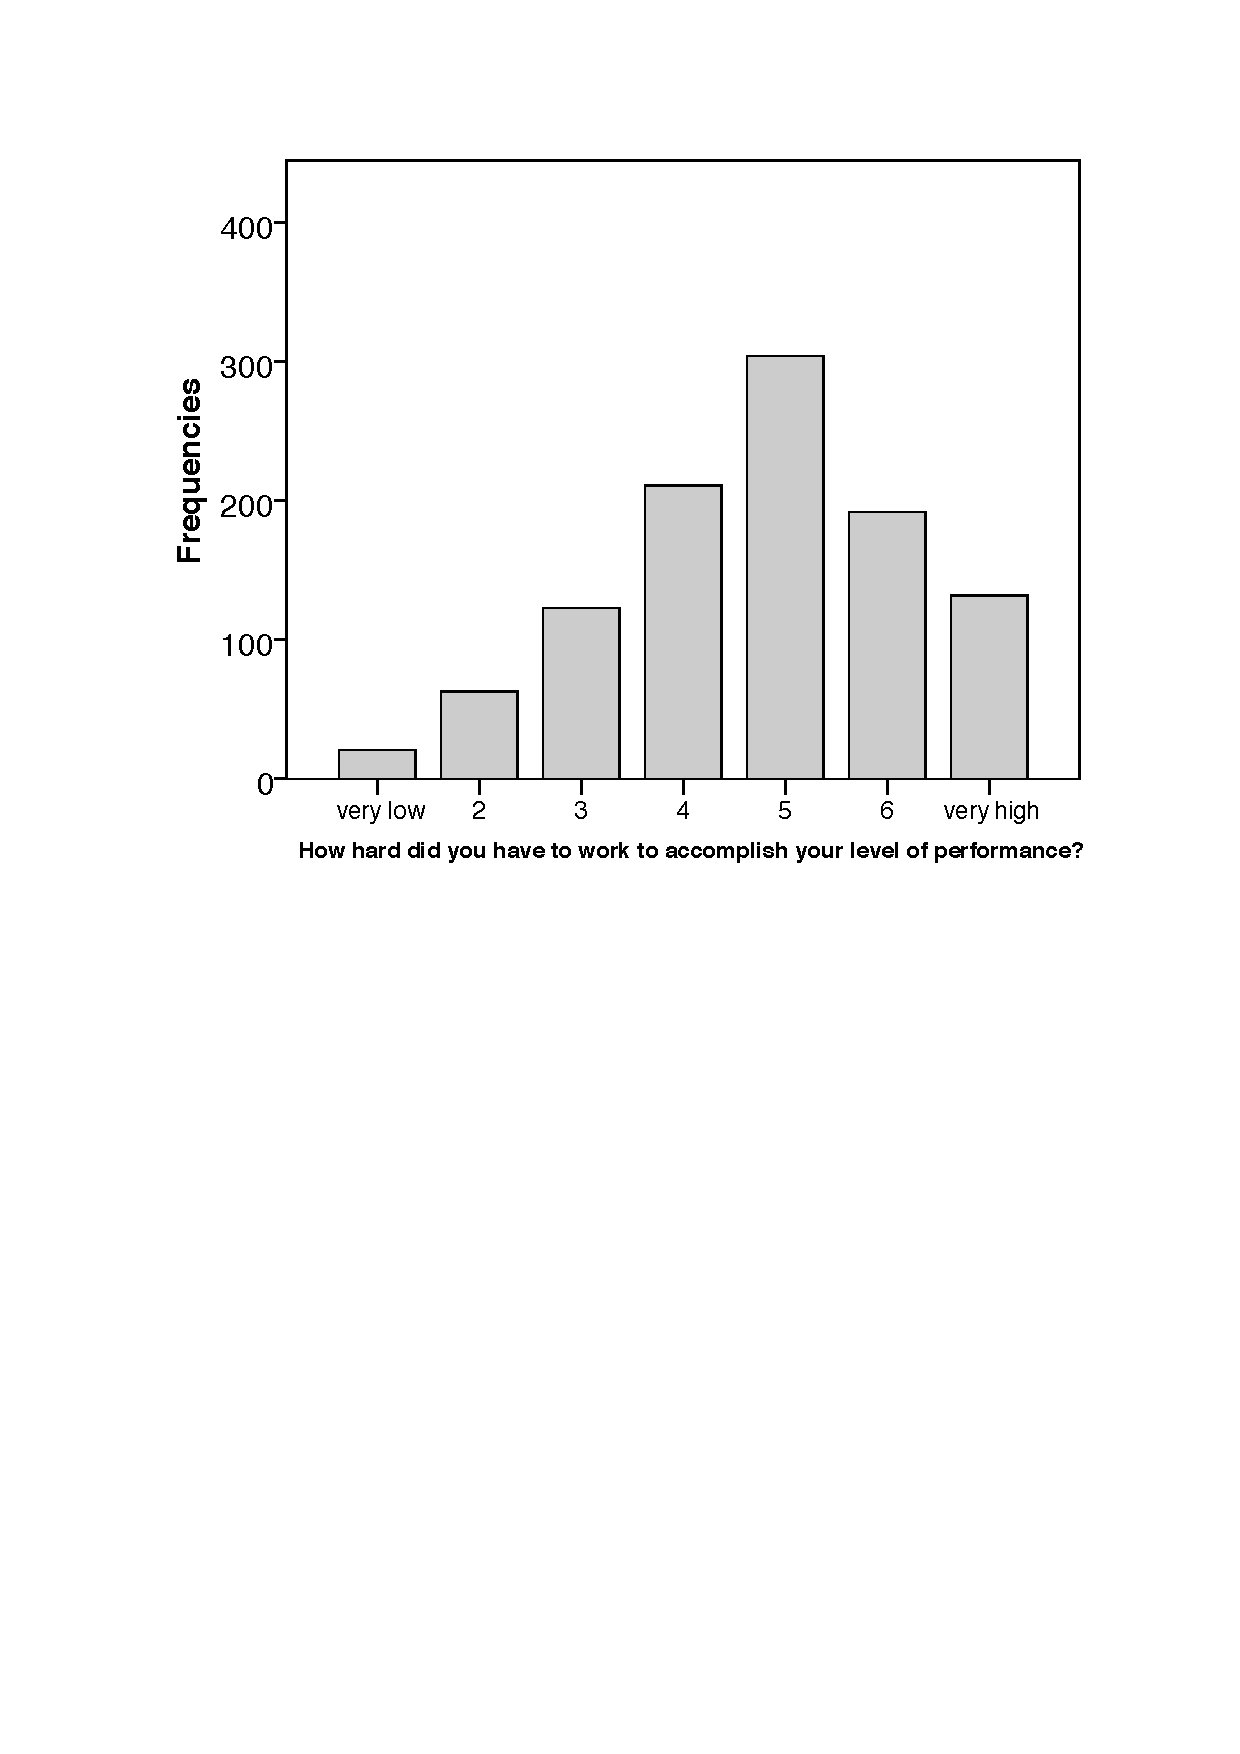
\includegraphics[height = 0.35\textwidth]{HistogramQuestion4.pdf}
\end{subfigure} 
\begin{subfigure} 
\centering
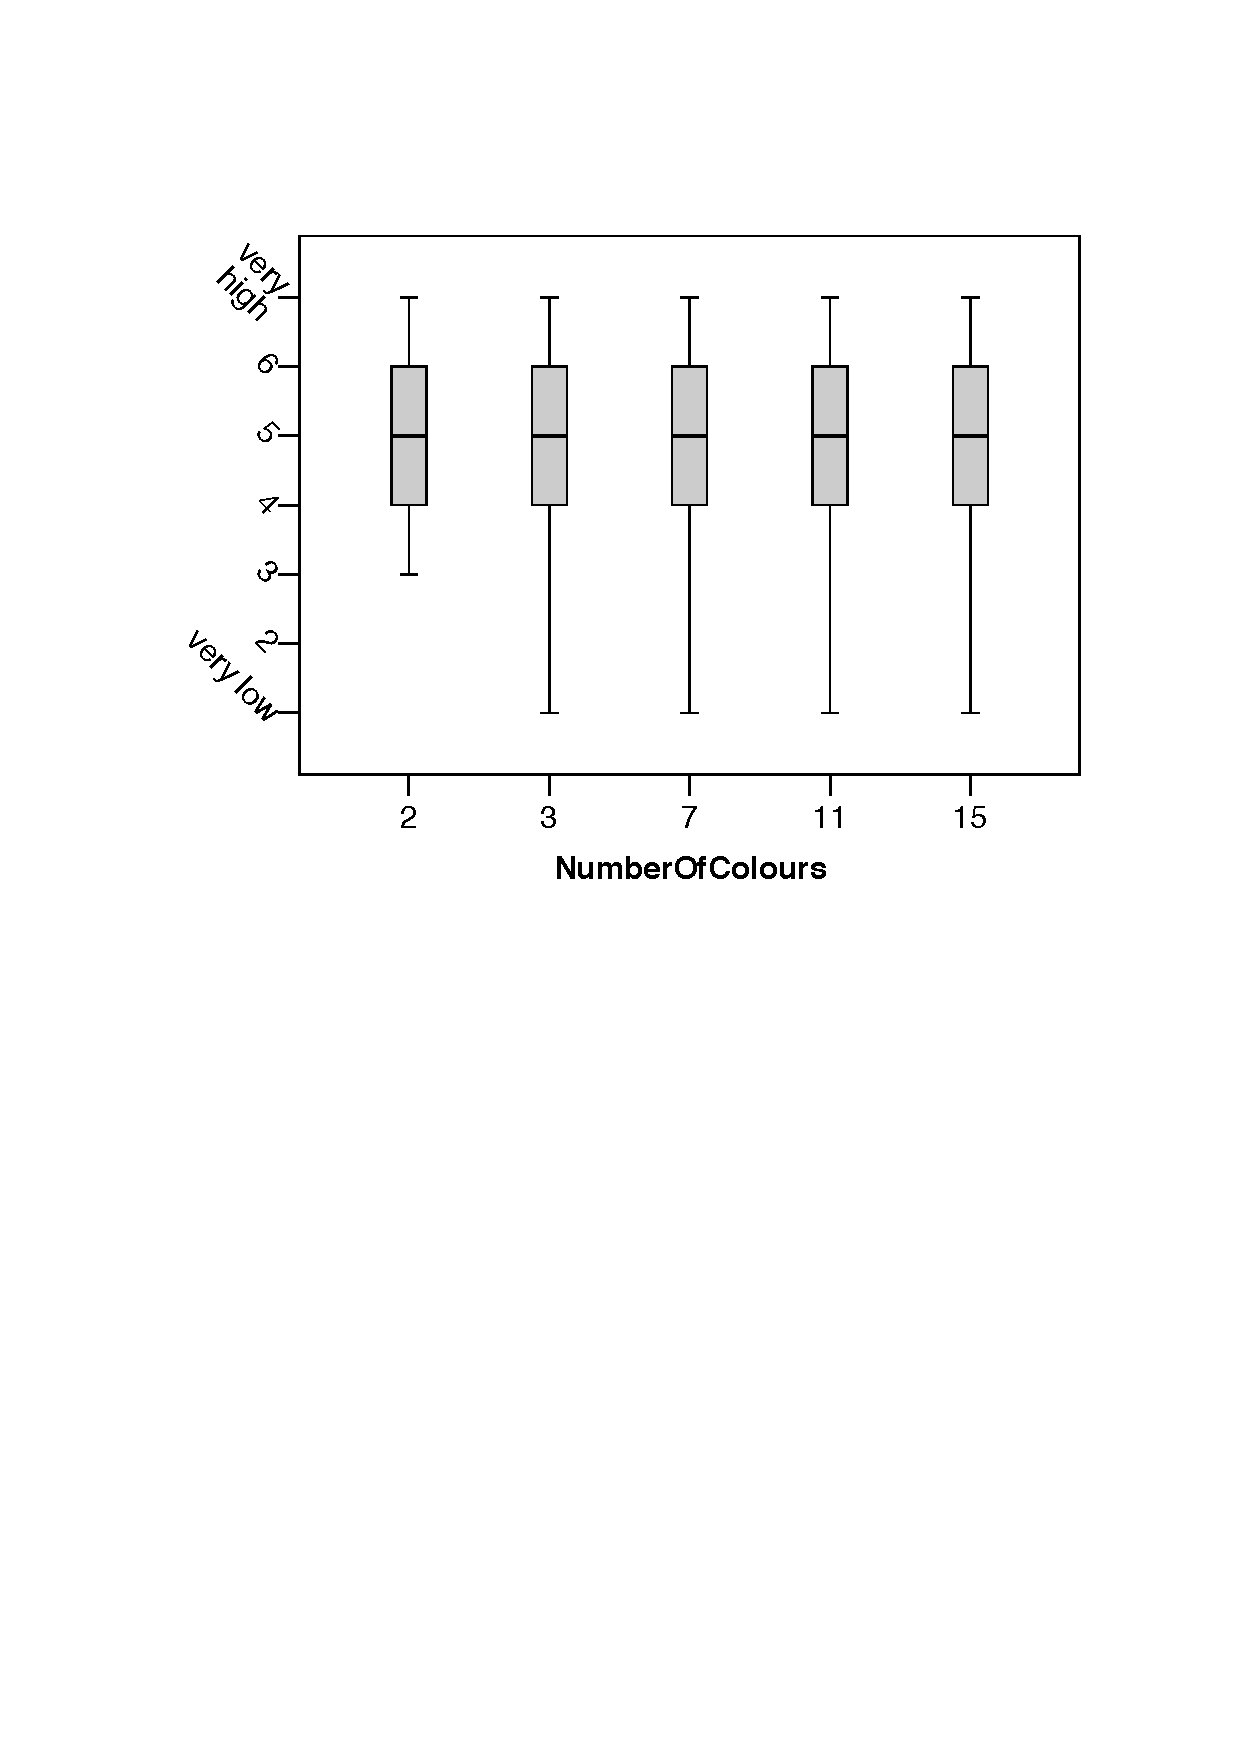
\includegraphics[height = 0.35\textwidth]{BoxplotQuestion4.pdf}
\end{subfigure}
  \caption[Question 4 - Histogram and Box plot]{Question 4 - very low (1) to very high (7}
    \label{Question4} 
\end{center}
\end{figure}
\begin{figure}[htbp] % Question5	
\begin{center} 
\begin{subfigure} 
\centering
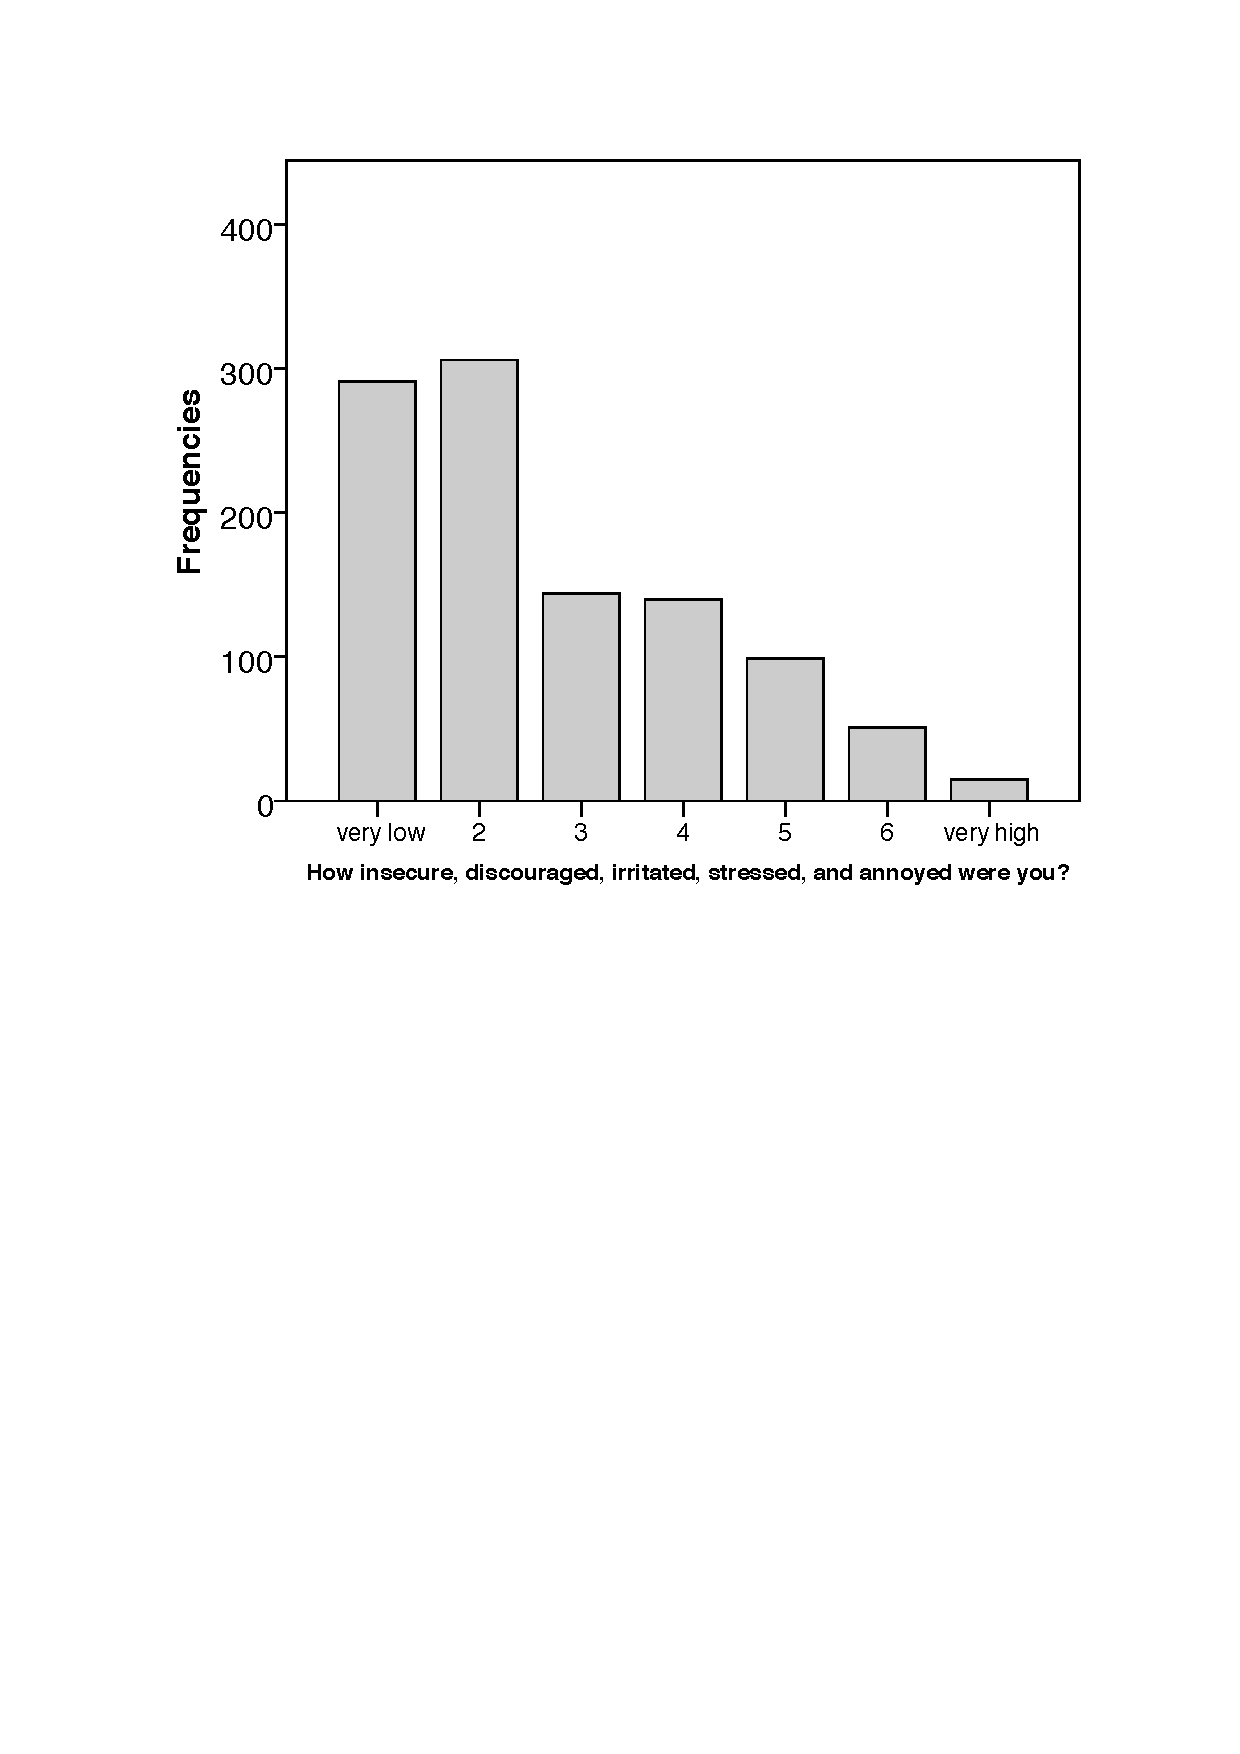
\includegraphics[height = 0.35\textwidth]{HistogramQuestion5.pdf}
\end{subfigure} 
\begin{subfigure} 
\centering
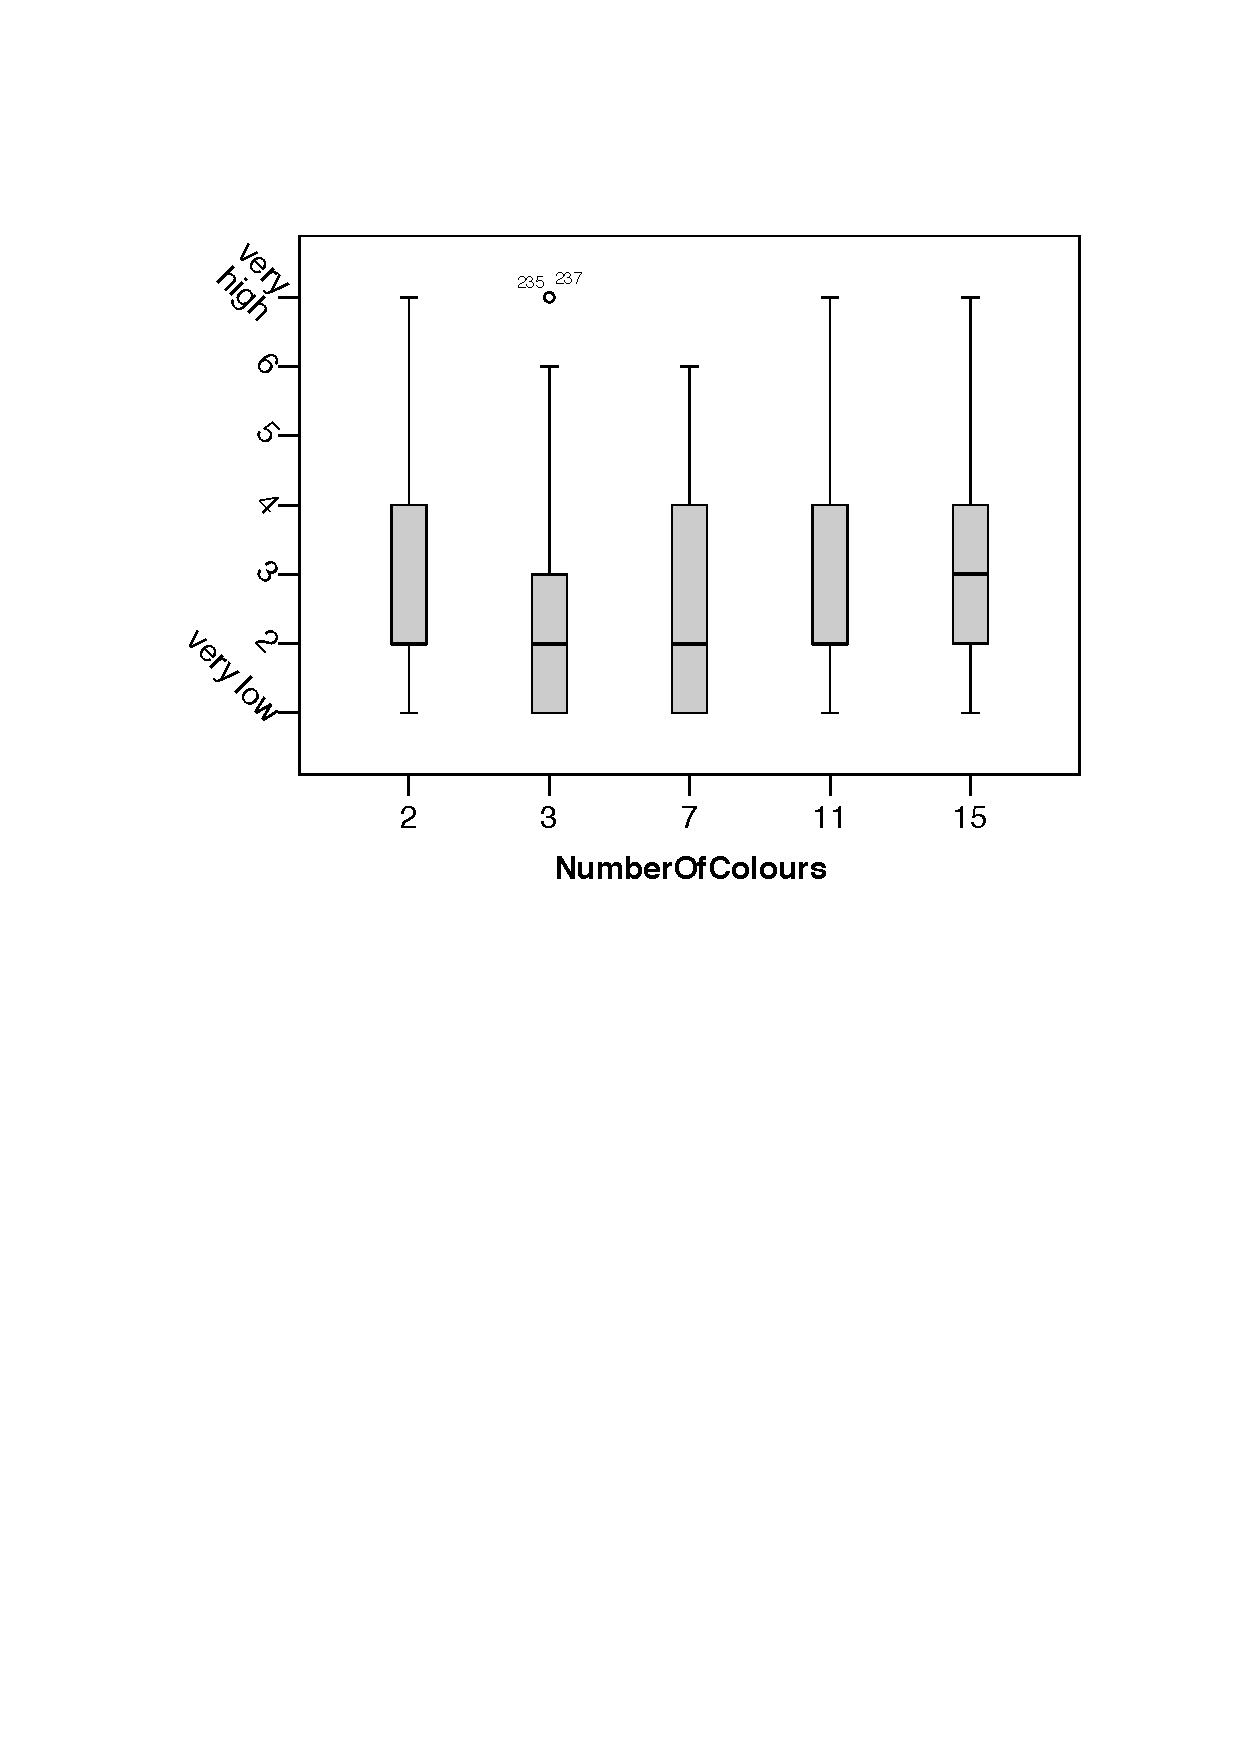
\includegraphics[height = 0.35\textwidth]{BoxplotQuestion5.pdf}
\end{subfigure}
  \caption[Question 5 - Histogram and Box plot]{Question 5 - very low (1) to very high (7)}
    \label{Question5} 
\end{center}
\end{figure}


